\chapter{โครงข่ายประสาทเทียม}
\label{chapter: ANN}
\index{Artificial Neural Network}
\index{โครงข่ายประสาทเทียม}

\begin{verse}
``Alone we can do so little. Together we can do so much.''\\
--- Helen Keller
\end{verse}

\begin{verse}
``ลำพังเราทำได้น้อยนิด รวมกันเราทำได้มากมาย''\\
--- เฮเลน เคลเลอร์
\end{verse}

%\begin{verse}
%``No one can whistle a symphony. It takes a whole orchestra to play %it.''
%H.~E.~Luccock
%\end{verse}

บทที่~\ref{chapter: Linear Models} อภิปรายโมเดลเชิงเส้น สำหรับการหาค่าถดถอยและการจำแนกประเภท. โมเดลเชิงเส้นกับเบซิสฟังชั่นแบบพหุนาม ถึงแม้จะมีคุณสมบัติดีๆหลายอย่าง เช่น 
ค่าพารามิเตอร์ของโมเดลเหล่านี้สามารถหาได้ง่าย 
แต่การนำไปใช้งานจริงกลับมีข้อจำกัดมาก โดยเฉพาะอย่างยิ่งในแง่ของคำสาปของมิติ.

%\begin{minipage}{5.5in}
{\small
\begin{shaded}
\textit{คำสาปของมิติ} (Curse of Dimensionality)
กล่าวถึง ปัญหาของ\textit{คุณสมบัติการขยาย} (scalability) ที่เมื่อตัวแปรมีมิติสูงขึ้น ปริมาณการคำนวณที่ต้องการจะมีเพิ่มขึ้นอย่างมากมหาศาลรวมขึ้นความยุ่งยากอื่นๆ.
ตัวอย่างเช่น การแบ่งกลุ่ม หากเลือกใช้ดีกรีหนึ่ง
เช่น 
$\bm{\phi}(\mathbf{x} = [x_1, x_2]^T) = [x_1, x_2]^T$
\textit{เส้นแบ่งตัดสินใจ}(decision boundary) จะเป็นแค่เส้นตรงธรรมดา
ซึ่งหาก ข้อมูลมีความสัมพันธ์ระหว่างมิติ ดังแสดงในรูป~\ref{fig: ANN nonlinear decision boundary}
หากต้องการเส้นแบ่งตัดสินใจที่ยืดหยุ่นกว่าเส้นตรง เราอาจจะใช้เบซิสฟังชั่นดีกรีที่สูงขึ้น เช่น
$\bm{\phi}(\mathbf{x} = [x_1, x_2]^T) = [x_1,\; x_2,\; x_1^2,\; x_1 \cdot x_2,\; x_2^2]^T$
หรือดีกรีสาม $\bm{\phi}(\mathbf{x} = [x_1, x_2]^T) = [$ $x_1,\;$ $x_2,\; x_1^2,\;$ $x_1 \cdot x_2,\;$ $x_2^2,\;$ $x_1^3,\;$ $x_1^2 x_2,\;$ $x_1 x_2^2,\;$ $x_2^3]^T$.
สังเกตุ ถ้าข้อมูลทีมิติมากขึ้น เช่น $\bm{\phi}([x_1, x_2, x_3]^T) = [x_1,\; x_2,\; x_3,\; x_1^2,\; x_1 x_2,\; x_1 x_3,\; x_2^2,\; x_2 x_3,\; x_3^2,\; x_1^3,\; x_1 x_2^2,\; x_1 x_2 x_3,\; x_1^2 x_2,\; \ldots,\; x_3^3]^T$
แล้วจินตนาการถึงการทำดีกรีที่สูงขึ้นไปอีก หรือ เมื่อข้อมูลมีมิติที่มากขึ้นอีก 
ความซับซ้อนของสมการจะเพิ่มขึ้นไปอย่างมากมายจนยากจะจัดการได้.
\end{shaded}
}
%\end{minipage}

แนวทางหนึ่งที่จะช่วยบรรเทาปัญหาคำสาปของมิติได้บ้าง ก็คือการเลือกใช้เบซิสฟังชั่นที่ปรับตัวเองได้.
กล่าวคือ เบซิสฟังชั่นก็มีพารามิเตอร์ที่ปรับตัวเองได้.
โมเดลที่เป็นที่รู้จักดีในแนวคิดนี้คือโครงข่ายประสาทเทียม ซึ่งที่ชนิดที่นิยมก็คือ เพอร์เซปตรอนหลายชั้น.

%บางโมเดลเลือกใช้แนวทางที่
%เพื่อใช้โมเดลกับปัญหาขนาดใหญ่ได้ คือ
%ยอมให้เบซิสฟังชั่นปรับตามข้อมูลได้.
%ซึ่งเป็นแนวคิดของเครื่องเวกเตอร์สนับสนุน Support Vector Machine (SVM), ที่เราจะคุยกันในรายละเอียดที่หัวข้อ~\ref{sec: SVM},
%เครื่องเวกเตอร์สนับสนุน จะกำหนดเบซิสฟังชั่น ตามจุดข้อมูล ที่นำมาใช้ฝึกโมเดล 
%จำนวนเบซิสฟังชั่น ของ เครื่องเวกเตอร์สนับสนุน จะขึ้นกับจุดข้อมูลที่เลือกมา ซึ่งปกติแล้วจะมีจำนวนมาก และ จำนวนเบซิสฟังชั่นก็จะแปรตามขนาดของชุดข้อมูลทที่นำมาฝึกโมเดลอีกด้วย
%อีก

%
\begin{figure}
\begin{center}
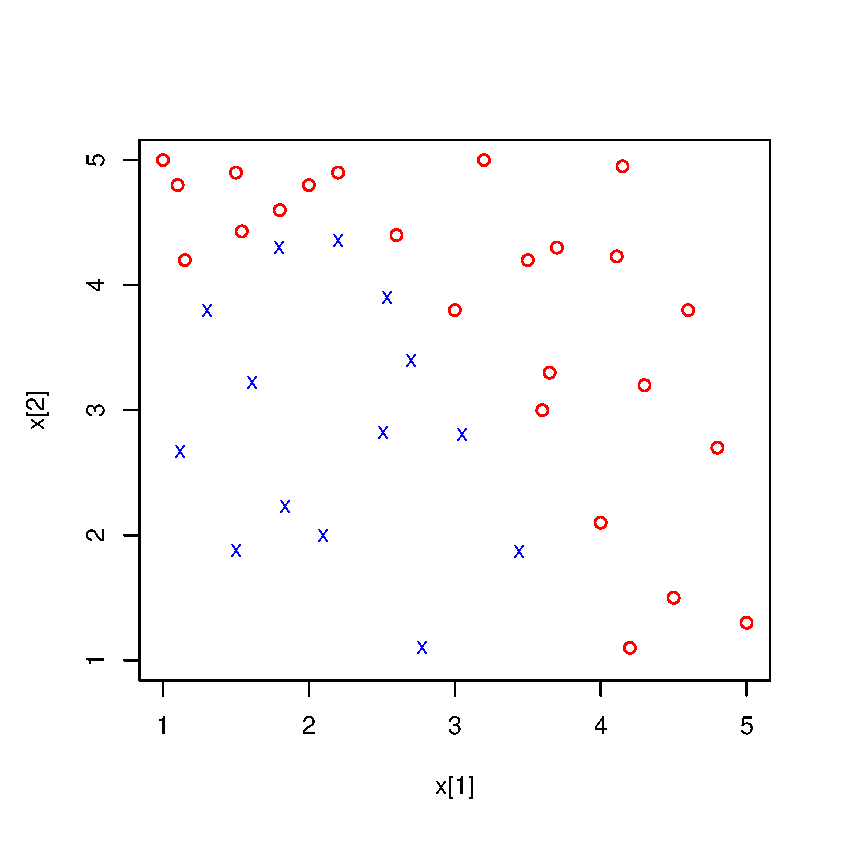
\includegraphics[height=3in]{04ANN/quadraticDecisionBound.eps}
\end{center}
\caption{ตัวอย่างข้อมูลที่เส้นแบ่งตัดสินใจเกินดีกรีเชิงเส้น 
จุดข้อมูลจากกลุ่ม 1 แสดงด้วยวงกลม 
จุดข้อมูลจากกลุ่มที่ 2 แสดงด้วยกากบาท}
\label{fig: ANN nonlinear decision boundary}
\end{figure}
%

\section{เพอร์เซปตรอนหลายชั้น}
\label{sec: Multilayer Perceptron}

แนวคิดของ\textit{เพอร์เซปตรอนหลายชั้น} (Multi-Layer Perceptron ตัวย่อ MLP) เริ่มมาจาก การพยายามสร้างระบบที่เลียบแบบการทำงานของเซลล์ประสาทของสิ่งมีชีวิต 
(รูป~\ref{fig: ANN neuron} แสดงโครงสร้างเซลล์ประสาททั่วๆไป).
%
ปี 1957 แฟรงค์ โรเซนแบลท (Frank Rosenblatt) ได้สาธิตการทำงานของเซลล์ประสาทจำลอง  ด้วยเครื่องคอมพิวเตอร์
และ โรเซนแบลทเรียกเซลล์ประสาทจำลองนั้นว่า \textit{เพอร์เซปตรอน} (perceptron).
แนวคิดของเพอร์เซปตรอน คือการใช้หน่วยคำนวณง่ายๆ หลายๆหน่วย ต่อกันเป็นโครงข่าย และผลรวมของมันสามารถทำการคำนวณที่ซับซ้อนได้.

รูป~\ref{fig: ANN perceptron} แสดงโครงสร้างของเพอร์เซปตรอน.
การคำนวณของเพอร์เซปตรอน ก็คือจะนำเอาอินพุตแต่ละตัวไปคูณกับค่าน้ำหนักของอินพุตนั้นๆ 
และนำค่าผลคูณทั้งหมดมาบวกกัน
แล้วหากผลบวกมีค่ามากพอ นั่นคือเกิน\textit{ค่าระดับกระตุ้น} (threshold) เพอร์เซปตรอนจะอยู่ในสถานะถูกกระตุ้น (ให้เอาต์พุตเป็น $1$)
แต่หากผลบวกมีค่าต่ำกว่าระดับกระตุ้น 
เพอร์เซปตรอนจะอยู่ในสถานะไม่ถูกกระตุ้น (ให้เอาต์พุตเป็น $0$).
ดังนั้น เอาต์พุตของเพอร์เซปตรอน สามารถเขียนเป็นสมการได้ว่า
\[
   y = \left\{
     \begin{array}{l l}
        0 & \quad \mbox{เมื่อ} \quad w_1 x_1 + \ldots + w_D x_D < \tau \\
        1 & \quad \mbox{เมื่อ} \quad w_1 x_1 + \ldots + w_D x_D \geq \tau
     \end{array} \right.
\]
เมื่อ $w_1, \ldots, w_D$ เป็นน้ำหนักของอินพุต $x_1, \ldots, x_D$ ตามลำดับ,
$\tau$ คือ ค่าระดับกระตุ้้น,
และ ให้ $1$ แทน ค่าแสดงสถานะถูกกระตุ้น และ $0$ แทน สถานะไม่ถูกกระตุ้น.

เพื่อความสะดวก เรานิยาม \textit{ไบอัส} (bias) เป็น $b = -\tau$ และ เราจะได้
\[
   y = \left\{
     \begin{array}{l l}
        0 & \quad \mbox{เมื่อ} \quad  w_1 x_1 + \ldots + w_D x_D + b < 0 \\
        1 & \quad \mbox{เมื่อ} \quad w_1 x_1 + \ldots + w_D x_D + b \geq 0
     \end{array} \right.
\]
ซึ่งทำให้เราเขียนได้เป็น
\begin{eqnarray}
   y = f\left( \sum_i w_i x_i + b \right)
\label{eq: ANN perceptron}
\end{eqnarray}
เมื่อ เรานิยามฟังชั่น $f(\cdot)$ เป็น\textit{ฟังชั่นจำกัดแข็ง} (hard limit function),
\begin{eqnarray}
   f(a) = \left\{
     \begin{array}{l l}
        0 & \quad \mbox{เมื่อ} \quad a < 0,\\
        1 & \quad \mbox{เมื่อ} \quad a \geq 0.
     \end{array} \right.
\label{eq: ANN hard limit}
\end{eqnarray}
เนื่องจากฟังชั่นนี้จะให้ค่าสถานะการกระตุ้นของเพอร์เซปตรอน ฟังชั่นนี้จึงมักถูกเรียกว่า \textit{ฟังชั่นการกระตุ้น} (activation function).

สมการ~\ref{eq: ANN perceptron} จะเข้ากับ แผนภาพในรูป~\ref{fig: ANN perceptron} โดยอินพุต \verb|1, x[1], ..., x[D]| จะคูณกับน้ำหนัก \verb|b, w[1], ..., w[D]| ตามลำดับ
และ ผลคูณจะถูกนำมารวมกัน ก่อนที่จะผ่านไปเข้าฟังชั่นการกระตุ้น \verb|f| ที่จะให้ค่าเอาต์พุต \verb|y| ออกมา.

%
\begin{figure}
\begin{center}
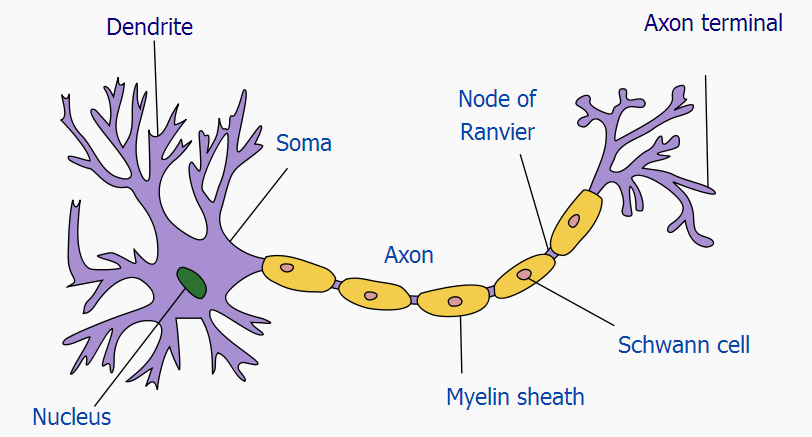
\includegraphics[height=3in]{04ANN/typicalNeuron.png}
\end{center}
\caption{รูปแสดงโครงสร้างของเซลล์ประสาททั่วๆไป
\textit{เดนไดรต์} (dendrite) ทำหน้าที่เสมือนอินพุตของเซลล์ 
และ \textit{แอกซอน} (axon) ทำหน้าที่เสมือนกับเอาต์พุตของเซลล์
{\footnotesize 
(ภาพจาก \texttt{http://en.wikipedia.org/wiki/File:Neuron\_Hand-tuned.svg})
}
}
%:////en.wikipedia.org//wiki//File:Neuron_Hand-tuned.svg}.}
\label{fig: ANN neuron}
\end{figure}
%

%
\begin{figure}
\begin{center}
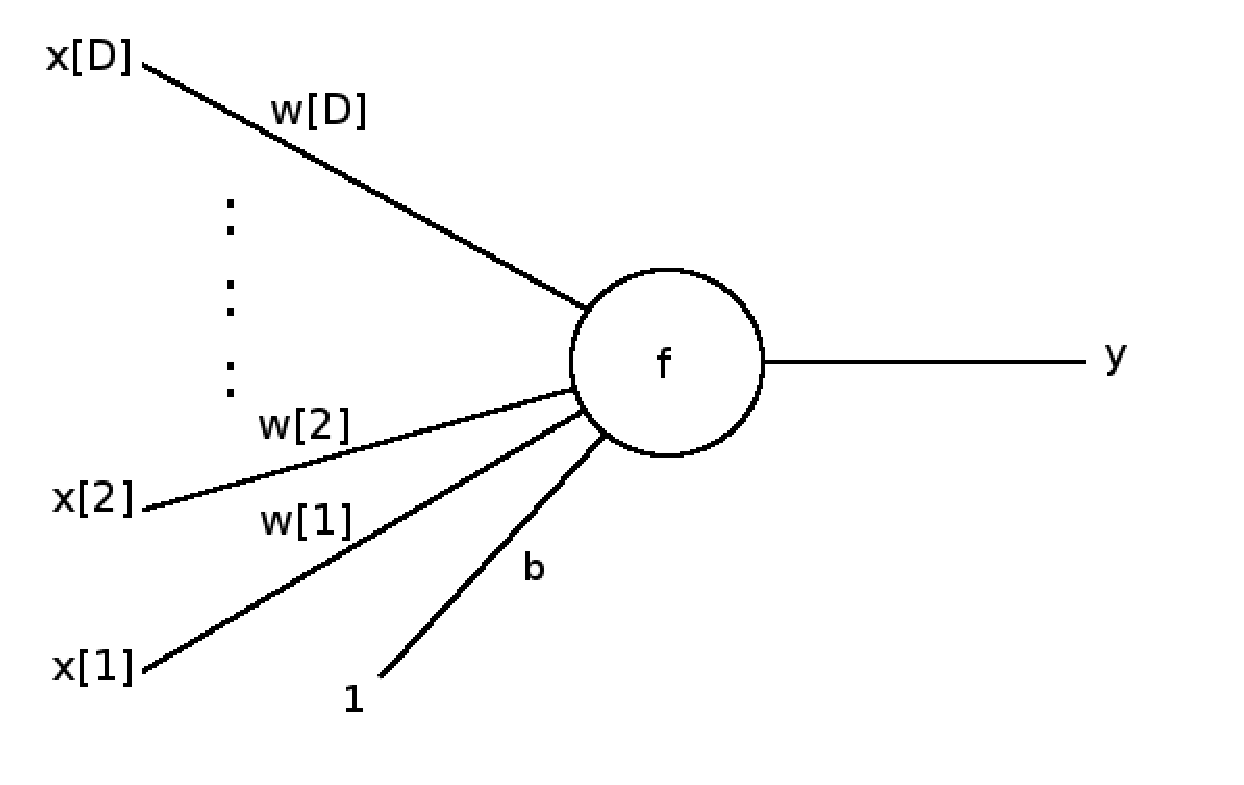
\includegraphics[height=3in]{04ANN/perceptron.eps}
\end{center}
\caption{แผนผังแสดงโครงสร้างของเพอร์เซปตรอน ซึ่ง เอาต์พุต \texttt{y = f(b + w[1] x[1] + ... + w[D]  x[D])} โดยฟังชั่น \texttt{f} จะเป็น\textit{ฟังชั่นจำกัดแข็ง} (hard limit function) สมการ~\ref{eq: ANN hard limit}}
\label{fig: ANN perceptron}
\end{figure}
%

%
%\begin{figure}
%\begin{center}
%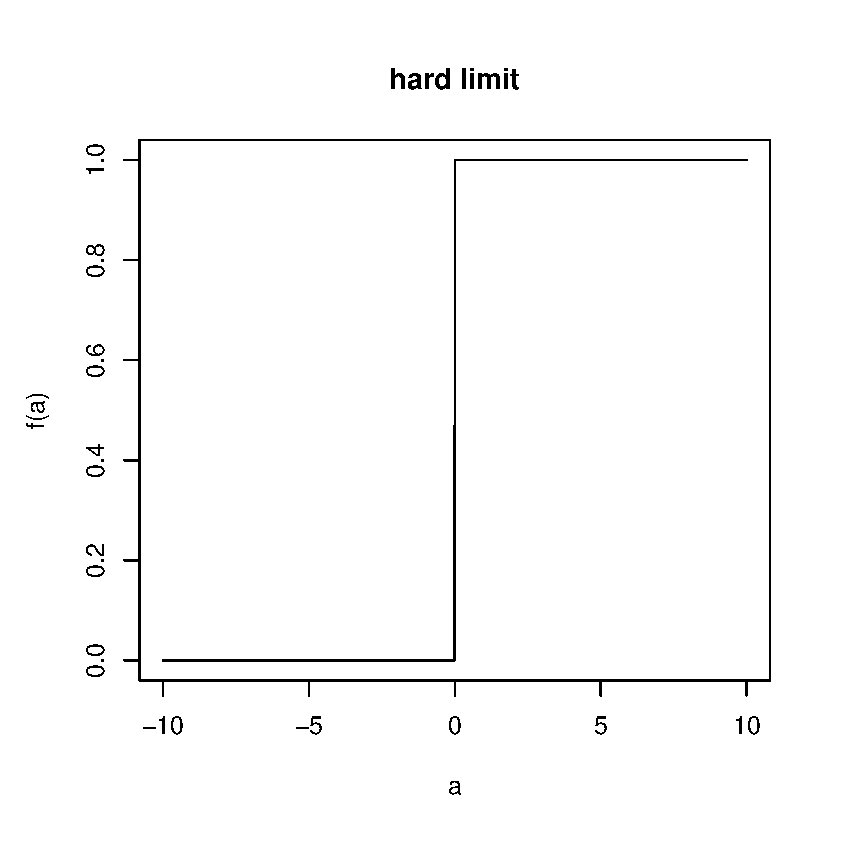
\includegraphics[height=3in]{04ANN/hardlim.eps}
%\end{center}
%\caption{ตัวอย่าง hard limit function ซึ่งเป็น activation function ของ perceptron: $f(a) = 1$ เมื่อ $a > 0$ และ $f(a) = 0$ เมื่อ $a < 0$.}
%\label{fig: ANN hard limit function}
%\end{figure}
%

ในตอนนั้น งานของโรเซนแบลททำให้วงการคอมพิวเตอร์ โดยเฉพาะอย่างยิ่งวงการปัญญาประดิษฐ์ตื่นเต้นมาก
ที่เราจะสามารถสร้างเครื่องจักรที่สามารถเลียบแบบการทำงานของสมองมนุษย์ได้
เกิดการคาดการณ์ถึงศักยภาพ ความสามารถต่างๆ ที่เครื่องคอมพิวเตอร์จะสามารถทำได้.
แต่ความฝันและความหวังก็ล่มสลายไป หลังจาก มาร์วิน มินสกี้ (Marvin Minsky) และ เซมัวร์ ปาเปิต (Seymour Papert) ได้ร่วมกันเขียนหนังสือเพอร์เซปตรอนส์\cite{MinskyPapert1969a} ที่วิเคราะห์โครงสร้างและการทำงานของเพอร์เซปตรอน.
ประเด็นสำคัญของหนังสือ คือ
มินสกี้และปาเปิตถกว่าเพอร์เซปตรอนนั้นสามารถทำได้แต่งานง่ายๆ 
เช่นหากเป็นงานการจำแนกประเภท ก็สามารถทำงานได้กับปัญหาที่สามารถแบ่งได้ด้วยเส้นแบ่งตัดสินใจเชิงเส้นเท่านั้น 
ไม่สามารถทำงานที่ซับซ้อนกว่านั้นได้.
พร้อมทั้งยังยกตัวอย่าง การทำงานของตรรกะ \textit{เอ็กซ์-ออร์} (XOR หรือ exclusive OR) ที่เพอร์เซปตรอนไม่สามารถเลียบแบบได้.
ตาราง~\ref{tbl: ANN XOR} แสดงพฤติกรรมของตรรกะเอ็กซ์-ออร์.

%
\begin{table}[hbtp]
\caption{ตรรกะ\textit{เอ็กซ์-ออร์} (XOR หรือ exclusive OR)}
\begin{center}
\begin{tabular}{|c|c|c|}
\hline 
$x_1$ & $x_2$ & $y$ \\
\hline
0     &    0  & 0   \\
0     &    1  & 1   \\
1     &    0  & 1   \\
1     &    1  & 0   \\
\hline
\end{tabular} 
\end{center}
\label{tbl: ANN XOR}
\end{table}


ผลของหนังสือเพอร์เซปตรอนส์ นอกจากจะทำให้เพอร์เซปตรอนเสื่อมความสนใจแล้ว 
ยังทำให้เทคนิคทางด้านโครงข่ายประสาทเทียมทั้งหมด รวมไปถึงสาขาวิชาปัญญาประดิษฐ์ 
เสียความนิยมและเสื่อมความสนใจไปในช่วงหลายปีต่อจากนั้น
จนเรียกกันว่า ช่วงเวลานั้นเป็น \textit{หน้าหนาวของปัญญาประดิษฐ์} (AI Winter).
%ช่วงนั้น ทุนวิจัย สำหรับงานด้านปัญญาประดิษฐ์ หาได้ยากมาก.
โครงข่ายประสาทเทียมเสียความนิยมไป 
จนกระทั่งหลายปีให้หลัง งานของเวอร์โบส\cite{Werbos1974a}และโดยเฉพาะอย่างยิ่งงานของกลุ่มของรูเมลาร์ต ฮินตัน และวิลเลี่ยม\cite{RumelhartEtAl1986a} ที่ออกมาแสดงให้เห็นถึงประสิทธิผลของโครงข่ายประสาทเทียม 
และนำเสนอวิธีการหาค่าพารามิเตอร์ที่มีประสิทธิภาพ 
ซึ่งงานเหล่านี้ ได้ช่วยฟื้นฟูความนิยมของโครงข่ายประสาทเทียมกลับมาใหม่.

เมื่อจะกล่าวไปแล้ว สิ่งที่มินสกี้กับปาเปิตถกว่า เพอร์เซปตรอนทำงานได้แต่งานง่ายๆ ก็ไม่ได้ผิดซะทั้งหมดนัก.
เพียงแต่ว่า มินสกี้กับปาเปิตสรุปความเห็น จากการวิเคราะห์การทำงานของ\textit{เพอร์เซปตรอนชั้นเดียว} (one-layer perceptron).
การทำงานของโครงข่ายสมองมนุษย์ไม่ได้เป็นชั้นเดียว 
ในลักษณะเดียวกันโครงข่ายประสาทเทียมที่มีประสิทธิผล จะต้องมีโครงสร้างมากกว่าหนึ่งชั้น.
นั่นก็คือ ที่มาของพัฒนาการต่อมา ได้แก่ \textit{เพอร์เซปตรอนหลายชั้น} (Multi-Layer Perceptron คำย่อ MLP) ซึ่งชื่อได้เน้นย้ำว่า มีการใช้โครงข่ายประสาทเทียมหลายชั้น.

รูป~\ref{fig: ANN MLP for XOR} แสดง\textit{เพอร์เซปตรอนสองชั้น} (2-layer perceptron) ที่สามารถเลียนแบบการทำงานของตรรกะเอ็กซ์-ออร์ได้.
เอาต์พุตของเพอร์เซปตรอนชั้นแรก ซึ่งคือ $z_1 = f(-30 x_1 + 30 x_2 - 20)$ และ $z_2 = f(30 x_1 - 30 x_2 - 20)$
ทำหน้าที่เป็นอินพุตของเพอร์เซปตรอนชั้นที่สอง
และเอาต์พุตของเพอร์เซปตรอนชั้นที่สอง (และกรณีนี้ก็เป็นเอาต์พุตของโครงสร้างทั้งหมด) คือ $y = f(30 z_1 + 30 z_2 - 20)$.
และตาราง~\ref{tbl: ANN MLP for XOR} แจกแจงการทำงาน โดย $a^{(1)}_1$, $a^{(1)}_2$, $a^{(2)}$ เป็นผลรวมของน้ำหนักคูณอินพุตของเพอร์เซปตรอนชั้นที่หนึ่งตัวบน ตัวล่าง และชั้นที่สอง ตามลำดับ.
สังเกตุว่า เราสามารถเปลี่ยนค่าน้ำหนักของโครงข่ายประสาทเทียมไปใช้ค่าอื่นได้ โดยที่การทำงานยังคงเดิมได้ 
เช่น เราอาจใช้ค่า $20, -20, -10$ แทน $30, -30, -20$ ในรูปได้ โดยพฤติกรรมของโครงข่ายยังคงให้ผลความสัมพันธ์ระหว่างอินพุตกับเอาต์พุตคงเดิม.
ซึ่ง นี่คือลักษณะอย่างหนึ่งของโครงข่ายประสาทเทียม ที่ ค่าน้ำหนักที่ดีที่สุดของโครงข่ายประสาทเทียมมีได้หลายชุด.

%\begin{minipage}{5.5in}
{\small
\begin{shaded}
หากมองจากทฤษฎีการหาค่าดีที่สุด  
ปัญหาการหาค่าน้ำหนักที่ดีที่สุดของโครงข่ายประสาทเทียม จะเป็นปัญหาในลักษณะที่เรียกว่า \textit{ปัญหาที่ไม่เป็นคอนเวกซ์} (non-convex problem)
ซึ่งการหาค่าน้ำหนักที่ดีที่สุดในปัญหาแบบนี้จะทำได้ยาก.
%
ในทางปฏิบัติ การฝึกโครงข่ายประสาทเทียมก็คือการหาค่าน้ำหนักที่ดี 
แต่ไม่อาจรับประกันได้เลยว่าเราจะได้ค่าน้ำหนักที่ดีที่สุด 
ซึ่งเรื่องนี้เป็นลักษณะอย่างหนึ่งที่ผู้ใช้โครงข่ายประสาทเทียมมักสะท้อนออกมาว่า
%ให้ความเห็นว่า
โครงข่ายประสาทเทียมนั้นฝึกยาก
\end{shaded}
}
%\end{minipage}

%
\begin{figure}
\begin{center}
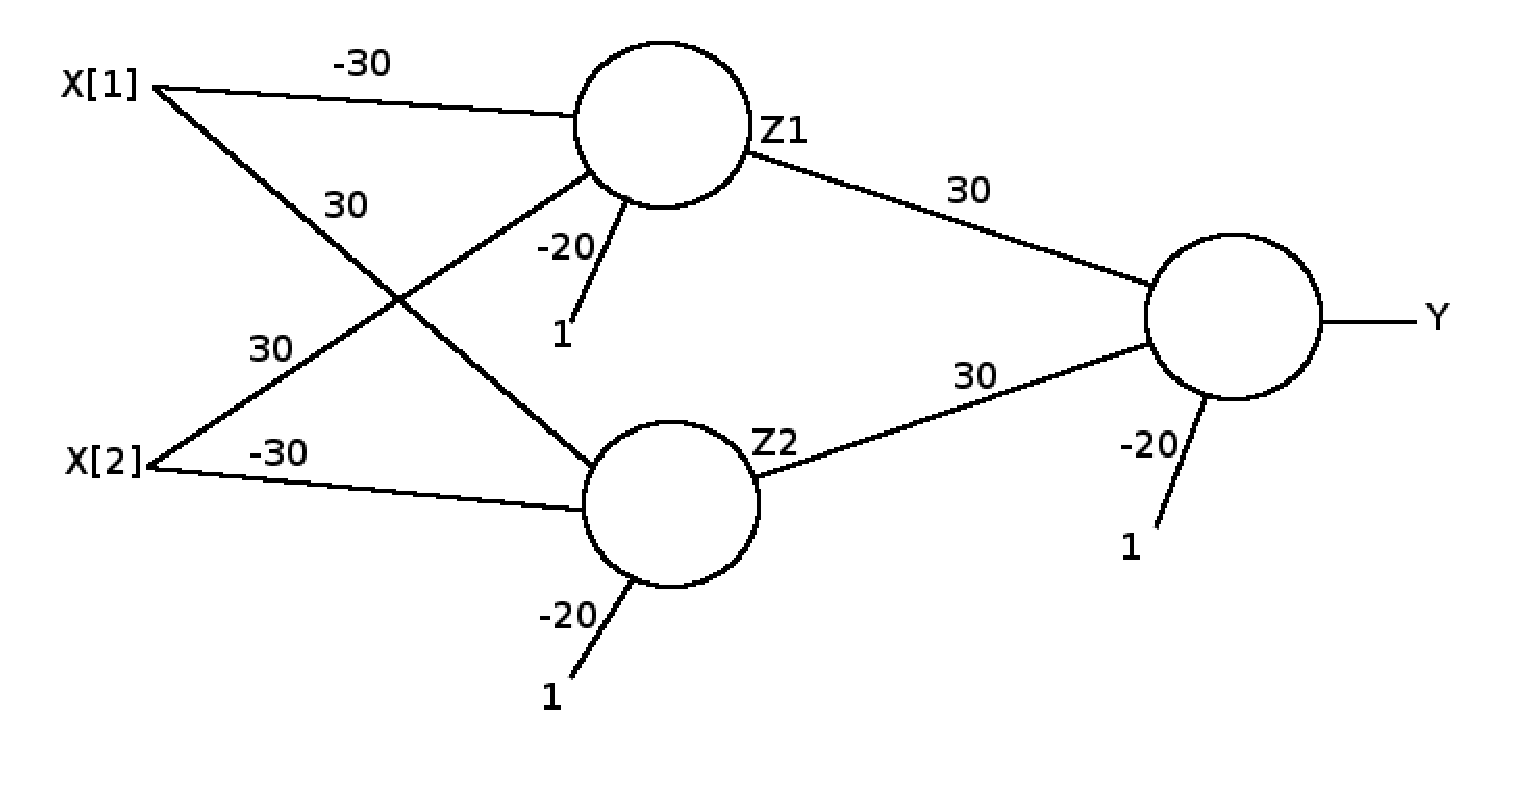
\includegraphics[height=3in]{04ANN/MLPXor.eps}
\end{center}
\caption{โครงข่ายเพอร์เซปตรอนที่ทำงานเลียบแบบตรรกะเอ็กซ์-ออร์ได้.}
\label{fig: ANN MLP for XOR}
\end{figure}
%

%
\begin{table}[hbtp]
\caption{การทำงานในแต่หน่วยของเพอร์เซปตรอน $2$ ชั้นในรูป~\ref{fig: ANN MLP for XOR}}
{\tiny %\scriptsize
\begin{center}
\begin{tabular}{|c|c|c|c|c|c|c|c|}
\hline 
$x_1$ & $x_2$ 
 & $a^{(1)}_1$ & $z_1$ 
 & $a^{(1)}_2$ & $z_2$ 
 & $a^{(2)}$ & $y$ \\
\hline
$0$     &    $0$  
& $-30 (0) + 30 (0) - 20$   & $f(-20)$
& $30 (0) - 30 (0) - 20$   & $f(-20)$
& $30 (0) + 30 (0) - 20$  & $f(-20)$ \\
& 
& $= -20$ & $= 0$
& $= -20$ & $= 0$
& $= -20$ &  $= 0$ \\
\hline
$0$     &    $1$  
& $-30 (0) + 30 (1) - 20$   & $f(10)$
& $30 (0) - 30 (1) - 20$   & $f(-50)$
& $30 (1) + 30 (0) - 20$  & $f(10)$ \\
& 
& $= 10$ & $= 1$
& $= -50$ & $= 0$
& $= 10$ &  $= 1$ \\
\hline
$1$     &    $0$  
& $-30 (1) + 30 (0) - 20$   & $f(-50)$
& $30 (1) - 30 (0) - 20$   & $f(10)$
& $30 (1) + 30 (0) - 20$  & $f(10)$ \\
& 
& $= -50$ & $= 0$
& $= 10$ & $= 1$
& $= 10$ &  $= 1$ \\
\hline
$1$     &    $1$  
& $-30 (1) + 30 (1) - 20$   & $f(-20)$
& $30 (1) - 30 (1) - 20$   & $f(-20)$
& $30 (0) + 30 (0) - 20$  & $f(-20)$ \\
& 
& $= -20$ & $= 0$
& $= -20$ & $= 0$
& $= -20$ &  $= 0$ \\
\hline
\end{tabular} 
\end{center}
}%end /small
\label{tbl: ANN MLP for XOR}
\end{table}

%
ปัจจุบันโครงข่ายประสาทเทียมเป็นโมเดลได้ถูกนำไปใช้อย่างกว้างขวาง ในงานหลายๆลักษณะ เช่น การหาค่าถดถอย การจำแนกประเภท การประมาณฟังชั่น และในแอพพลิเคชั่นต่างๆ รวมถึงงานการประมวลผลภาพและงานการประมวลผลเสียงพูด.
% image processing และ speech processing.
%
นอกจากนั้น มีการศึกษาโครงข่ายประสาทเทียมในทางทฤษฎี และพิสูจน์ว่าโครงข่ายประสาทเทียมเป็น\textit{ตัวประมาณค่าสากล} (universal approximator)\cite{Cybenko1989a, Hornik1991a}
ซึ่งความหมายคือ 
โครงข่ายประสาทเทียมสามารถแทนฟังชั่นใดๆก็ได้ ที่ความละเอียดตามที่ต้องการ หากมีจำนวนหน่วยคำนวณมากเพียงพอ.
ตามทฤษฎีแล้ว แค่โครงข่ายประสาทเทียมแบบสองชั้นก็เป็นตัวประมาณค่าสากลได้แล้ว.
%ก็สามารถที่ จะแทนฟังชั่นใดๆได้แล้ว หากมีจำนวนเพอร์เซปตรอนใน ชั้นที่ซ่อนไว้มากเพียงพอ.
%
%โครงข่ายประสาทเทียม $2$ ชั้น สามารถประมาณแทนฟังชั่นได้ทุกชนิด ในความละเอียดตามที่ต้องการได้ เพียงต้องมีจำนวน หน่วยประสาทเทียมที่มากเพียงพอเท่านั้น.

กลับมาที่เรื่องการหาค่าน้ำหนักที่เหมาะสมของโครงข่ายประสาทเทียม 
อย่างที่เห็นจากตัวอย่าง การที่จะทำให้โครงข่ายประสาทเทียมทำงานได้ตามต้องการได้นั้น 
นอกจากโครงข่ายจะต้องมีโครงสร้างที่รองรับได้แล้ว(มีจำนวนหน่วยคำนวณเพียงพอ) 
ค่าของน้ำหนักต่างๆจะต้องมีค่าที่เหมาะสมด้วย.
การหาค่าน้ำหนักของโครงข่ายประสาทเทียม เราสามารถทำได้ในลักษณะเดียวกับ การที่เราหาค่าพารามิเตอร์ของฟังชั่นพหุนามในหัวข้อ~\ref{section: Polynomial Curve Fitting}
นั่นคือการใช้วิธีของการหาค่าดีที่สุด.
รายละเอียดของกระบวนการหาค่าน้ำหนัก หรือมักนิยมเรียกว่าการฝึกโครงข่ายประสาทเทียม จะถกในหัวข้อ~\ref{sec: ANN training}.

ก่อนจะศึกษากระบวนการหาค่าน้ำหนัก มีประเด็นที่น่าสนใจที่ควรกล่าวถึงก่อน 
นั่นคือการหาอนุพันธ์เป็นเครื่องมือสำคัญอย่างหนึ่ง สำหรับวิธีของการหาค่าดีที่สุด.
เพอร์เซปตรอนใช้ฟังชั่นกระตุ้นเป็นฟังชั่นจำกัดแข็ง
แต่เนื่องจาก ฟังชั่นจำกัดแข็ง(สมการ~\ref{eq: ANN hard limit}) เป็นฟังชั่นที่มีค่าไม่ต่อเนื่อง (ที่ $a = 0$) ทำให้ เราไม่สามารถหาค่าอนุพันธ์ของฟังชั่นจำกัดแข็งได้ ส่งผลให้การหาค่าน้ำหนักที่เหมาะสมของเพอร์เซปตรอนทำได้ยาก.

ฟังชั่นจำกัดแข็ง แม้จะเลียนแบบการทำงานของเซลล์ประสาท แต่ลักษณะทางคณิตศาสตร์ของมันเป็นอุปสรรคที่สำคัญ.
การสร้างโมเดลทางคณิตศาสตร์เพื่อประโยชน์ในการทำความเข้าใจเซลล์ประสาททางชีวภาพ 
จะจัดอยู่ในขอบข่ายของ\textit{ประสาทวิทยาเชิงคำนวณ} (computational neuroscience) 
ซึ่งเป็นสาขาเฉพาะ และอยู่นอกเหนือจากขอบเขตของหนังสือเล่มนี้.
%
แม้กระนั้น ฟังชั่นจำกัดแข็งเองก็ไม่ได้อธิบายการทำงานของเซลล์ประสาททางชีวภาพได้อย่างเที่ยงตรงซะทีเดียว
นอกจากนั้น สิ่งที่ต้องการจริงๆในมุมมองทางวิศวกรรม ก็คือเครื่องมือที่ใช้งานได้ เช่น โมเดลที่มีความสามารถในการทำนายที่ดี เป็นต้น.
%ดังนั้นจึงไม่มีเหตุผล ที่จะยึดติดกับฟังชั่นจำกัดแข็ง.

การที่จะฝึกโครงข่ายประสาทเทียมที่ใช้ฟังชั่นจำกัดแข็งจะทำได้ยากมาก หรือไม่สามารถทำได้อย่างมีประสิทธิภาพ
%
เมื่อปัญหาอยู่ที่ฟังชั่นจำกัดแข็ง วิธีแก้อย่างหนึ่งก็คือ การผ่อนปรนฟังชั่นจำกัดแข็งลง
โดย แทนที่จะใช้ฟังชั่นจำกัดแข็ง ฟังชั่นที่ประมาณฟังชั่นจำกัดแข็งจึงถูกนำมาใช้แทน.
ฟังชั่นประมาณนั้นคือ \textit{ฟังชั่นซิกมอยด์} (sigmoid function หรือบางครั้งเรียก logistic function หรือ logistic sigmoid function).
ฟังชั่นซิกมอยด์ เป็นฟังชั่นค่าต่อเนื่อง ดังนั้นจึงสามารถหาอนุพันธ์ตลอดช่วงค่าของอินพุต.
เราอาจจะมองว่า ฟังชั่นซิกมอยด์เป็นการประมาณฟังชั่นจำกัดแข็ง ด้วยฟังชั่นที่ต่อเนื่องที่สามารถหาค่าอนุพันธ์ได้.
รูป~\ref{fig: ANN activation function} เปรียบเทียบค่าของฟังชั่นจากฟังชั่นจำกัดแข็งกับฟังชั่นซิกมอยด์

%\begin{minipage}{5.5in}
{\small
\begin{shaded}
การใช้ฟังชั่นซิกมอยด์เป็นพัฒนาการของโครงข่ายประสาทเทียมของยุคต้นๆ.
เมื่อความเข้าใจพื้นฐานทางคณิตศาสตร์ดีขึ้น แม้แต่การใช้ซิกมอยด์เองก็ถูกผ่อนปรนลงไป.
โดยเฉพาะอย่างยิ่ง 
งานยุคหลังของการศึกษาโครงข่ายประสาทเทียมแบบลึกที่พบว่า
ปัจจัยสำคัญอย่างหนึ่งที่ช่วยแก้อุปสรรคของการฝึกโครงข่ายแบบลึก 
ก็คือ การเปลี่ยนฟังชั่นกระตุ้นไปใช้\textit{ฟังชั่นเชิงเส้นควบคุม} (rectified linear) 
ที่มีช่วงพลวัตรดีกว่าซิกมอยด์ ซึ่งช่วยลด\textit{ปัญหาเกรเดียนต์เลือนหาย} (vanishing-gradient issue) ลงได้.
%บทที่~\ref{chapter: ANN deep learning} อภิปรายพัฒนาการในยุคของโครงข่ายประสาทเทียมแบบลึก
\end{shaded}
}
%\end{minipage}

อย่างไรก็ตามแม้ ชื่อของเพอร์เซปตรอนจะเชื่อมโยงกับฟังชั่นจำกัดแข็ง 
แต่ในทางปฏิบัติแล้ว ชื่อ\textit{เพอร์เซปตรอนหลายชั้น} (MLP) ก็มักจะอ้างถึงโครงข่ายประสาทเทียมที่ใช้ฟังชั่นซิกมอยด์เป็นฟังชั่นกระตุ้น%
\footnote{
\textit{ฟังชั่นไฮเปอร์บอลิกแทนเจนต์} (hyperbolic tangent function)
$\tanh(x) = (e^x - e^{-x})/(e^x + e^{-x})$ 
ก็เป็นอีกฟังชั่นที่นิยมนำมาใช้เป็นฟังชั่นกระตุ้นของโครงข่ายประสาทเทียม.
แต่เพื่อความกระชับ เราจะพูดถึงซิกมอยด์ฟังชั่นเพียงอย่างเดียว.
}

%
\begin{figure}
\begin{center}
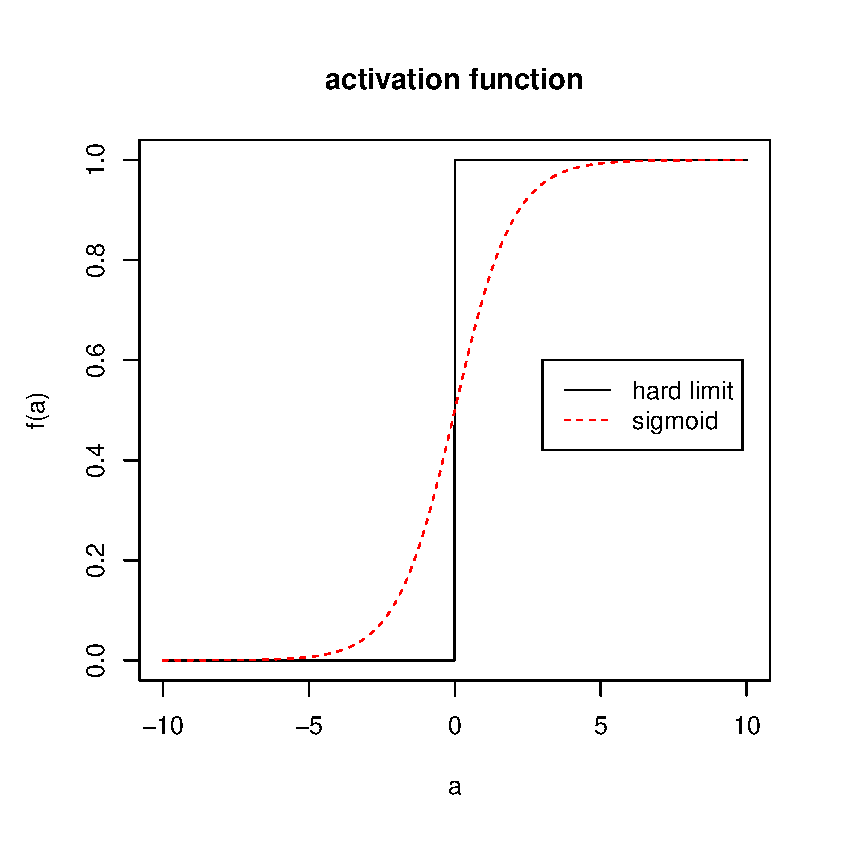
\includegraphics[height=3in]{04ANN/activation.eps}
\end{center}
\caption{ภาพเปรียบเทียบฟังชั่นจำกัดแข็งกับฟังชั่นซิกมอยด์}
\label{fig: ANN activation function}
\end{figure}
%

การอภิปรายข้างต้นถกถึงพัฒนาการของโครงข่ายประสาทเทียม
จากแรงบันดาลใจที่ได้จากการเลียนแบบเซลล์ประสาททางชีวภาพ 
มาเป็นโมเดลแบบเพอร์เซปตรอน 
จนพัฒนาต่อมาเป็นเพอร์เซปตรอนหลายชั้น.
ในทางปฏิบัติ การใช้งานโครงข่ายประสาทเทียมไม่จำเป็นต้องเข้าใจ หรือไปผูกภาพกับโครงข่ายประสาททางชีวภาพ
และการทำงานของโครงข่ายประสาทเทียมก็สามารถอธิบายได้เช่นเดียวกับโมเดลทางคณิตศาสตร์อื่นๆ.
หัวข้อ~\ref{sec: ANN structure} อธิบายโครงข่ายประสาทเทียม จากมุมมองของโมเดลทางคณิตศาสตร์
ที่ลักษณะเฉพาะของโครงข่ายประสาทเทียม สามารถเข้าไปช่วยแก้ปัญหาการสร้างโมเดลที่ยืดหยุ่นได้ ดังที่เกริ่นไว้ตอนต้น.

{\small
\begin{shaded}
\paragraph{\small เกร็ดความรู้สมองมนุษย์}
(เรียบเรียงจาก \cite{NIND} \cite{BuddhasBrain} และ \cite{Wikipedia})
\index{สมองมนุษย์}\index{Human Brain}
โดยเฉลี่ยแล้ว สมองมนุษย์มีขนาดประมาณ $1.13$ ถึง $1.26$ ลิตร และหนักประมาณ $1.3$ กก.
ใช้ออกซิเจนประมาณ $20$ เปอร์เซ็นของปริมาณทั้งหมดที่ร่างกายรับเข้าไป
และใช้กำลังงานประมาณ $25$ วัตต์\cite{GodwinCham2012a}.
%

สมองเชื่อมต่อกับส่วนอื่นๆของร่างกายผ่านไขสันหลัง 
%(สมองและไขสันหลังประกอบกันเป็น\textit{ระบบประสาทกลาง} (Central Nervous System คำย่อ CNS) 
และ\textit{ระบบประสาทนอกส่วนกลาง} (Peripheral Nervous System คำย่อ PNS) 
%
%และ\textit{ไขสันหลัง} (Spinal Cord)ประกอบกันเป็น\textit{ระบบประสาทกลาง} (Central Nervous System คำย่อ CNS).
ไขสันหลังทำหน้าที่หลักๆคือเชื่อมต่อสัญญาณควบคุมจากสมองไปยังส่วนต่างๆของร่างกาย และส่งผ่านสัญญาณรับรู้จากส่วนต่างๆของร่างกายกลับไปยังสมอง
และไขสันหลังเองก็มีระบบประสาทของตัวเองที่ช่วยทำงาน เช่นการควบคุมการตอบสนองฉับพลัน เป็นต้น.
ระบบประสาทนอกส่วนกลางมีหน้าที่หลักคือเชื่อมต่อสัญญาณจากสมองและไขสันหลังไปสู่อวัยวะต่างๆ.
%
%The spinal cord functions primarily in the transmission of neural signals between the brain and the rest of the body but also contains neural circuits that can independently control numerous reflexes and central pattern generators. The spinal cord has three major functions: as a conduit for motor information, which travels down the spinal cord, as a conduit for sensory information in the reverse direction, and finally as a center for coordinating certain reflexes.

การทำงานของสมองมีลักษณะคล้ายคณะกรรมการของกลุ่มผู้เชี่ยวชาญจำนวนมาก
นั่นคือ ส่วนต่างๆของสมองทำงานร่วมกัน แต่ว่าแต่ละส่วนของสมองมีหน้าที่เฉพาะด้าน.
เราอาจมองได้ว่าส่วนของสมองมีสามส่วนใหญ่ๆ คือ \textit{สมองส่วนบน} (forebrain), \textit{สมองส่วนกลาง} (midbrain), และ \textit{สมองส่วนล่าง} (hindbrain).

สมองส่วนล่างนับรวมส่วนบนของไขสันหลัง \textit{ก้านสมอง} (brain stem) และ \textit{เซเรเบลัม} (cerebellum).
สมองส่วนล่างจะควบคุมการทำงานที่เป็นพื้นฐานของการดำรงชีพ เช่น การหายใจ และการเต้นของหัวใจ.
เซเรเบลัมช่วยประสานงานเรื่องการเคลื่อนไหวและการเรียนรู้ของการเคลื่อนไหวที่เกิดจากการฝึกทำซ้ำๆ เช่น 
การเล่นเปียโนหรือการตีลูกเทนนิส จะอาศัยการทำงานของเซเรเบลัมช่วย.
%การฝึกการเคลื่อนไหวของศิลปะการต่อสู้ ที่ฝึกกระบวนท่าต่างๆซ้ำๆบ่อยๆ จนเกิดความชำนาญ

สมองส่วนกลางอยู่ด้านบนของก้านสมอง ทำหน้าที่เกี่ยวกับการควบคุมการตอบสนองแบบฉับพลัน และเป็นส่วนหนึ่งในระบบการควบคุมการเคลื่อนไหวของดวงตาและการเคลื่อนไหวโดยสมัครใจอื่นๆ.
สมองส่วนกลางนี้มีส่วนที่ทำงานประมวลผลภาพอยู่ด้วย.
\textit{สภาวะเห็นทั้งบอด} (blindsight) เป็นสภาวะของผู้พิการทางสายตา ที่การพิการเกิดจากส่วนประมวลผลภาพหลักที่\textit{เปลือกสมองส่วนการเห็น} (visual cortex ซึ่งจัดอยู่ในสมองส่วนบน)ไม่สามารถทำหน้าที่ได้ แต่ดวงตาและส่วนอื่นๆในระบบการมองเห็น รวมถึงส่วนประมวลผลภาพของสมองส่วนกลางยังดีอยู่.
สภาวะเช่นนี้ ตัวผู้พิการจะไม่รับรู้ถึงการมองเห็น 
แต่เมื่อมีการทดลอง
โดยบังคับให้ผู้มีสภาวะเห็นทั้งบอดบรรยายรูปร่างหรือตำแหน่งของวัตถุด้วยการเดา
ผู้มีสภาวะเห็นทั้งบอดจะบรรยายได้ถูกต้องทั้งรูปร่าง ตำแหน่ง และการเคลื่อนไหว
ซึ่งความถูกต้องแม่นยำที่ได้สูงมากเกินกว่าที่จะได้มาจากการคาดเดา.
คำอธิบายสภาวะนี้ก็คือ สมองกลับไปใช้ผลการประมวลภาพจากสมองส่วนกลาง ซึ่งแม้จะไม่มีความสามารถในการประมวลผลได้ดีเท่ากับเปลือกสมองส่วนการเห็น
แต่ก็ช่วยให้เกิดการมองเห็นใต้จิตสำนึกนี้เกิดขึ้นได้.

เนื่องจากระบบประมวลผลภาพในสมองมีทั้งที่สมองส่วนกลางและบริเวณเปลือกสมองส่วนการเห็นในสมองส่วนบน ทฤษฎีวิวัฒนาการเชื่อว่า
การประมวลภาพที่สมองส่วนกลางเป็นวิวัฒนาการในช่วงก่อน
(สัตว์หลายชนิด เช่น กบ ใช้การประมวลภาพที่สมองส่วนกลางเป็นหลัก)
และเปลือกสมองส่วนการเห็นเป็นวิวัฒนาการในช่วงต่อมา.
ผู้เชี่ยวชาญด้านประสาทวิทยาเดวิด ลินเดน (ผู้เขียนหนังสือ 
%\textit{จิตอุบัติ}
Accidental Mind\cite{Linden2008a}) ได้อธิบายเพิ่มเติมในการสนทนาส่วนตัวว่า
%ลินเดน อธิบายว่ากรณีที่เปลือกสมองส่วนการเห็นเสียหายแต่ส่วนอื่นๆดีอยู่ จะเป็นสภาวะเห็นทั้งบอด
หากการประมวลผลภาพของสมองส่วนกลางเสียหาย แต่ส่วนอื่นๆในระบบการมองเห็นยังดีอยู่ รวมถึงเปลือกสมองส่วนการเห็นก็ยังดีอยู่
ผู้ป่วยจะรับรู้ถึงการมองเห็นได้ แต่พบว่าผู้ป่วยจะมีการตอบสนอง\textit{การประสานงานระหว่างมือและตา} (hand-eye coordination) ที่ช้าลงอย่างชัดเจน.


%Researchers applied the same type of tests that were used to study blindsight in animals to a patient referred to as DB. The normal techniques that were used to assess visual acuity in humans involved asking them to verbally describe some visually recognizable aspect of an object or objects. DB was given forced-choice tasks to complete instead. This meant that even if he or she wasn't visually conscious of the presence, location, or shape of an object they still had to attempt to guess regardless. The results of DB's guesses—if one would even refer to them as such—showed that DB was able to determine shape and detect movement at some unconscious level, despite not being visually aware of this. DB themselves chalked up the accuracy of their guesses to be merely coincidental.[

สมองส่วนบนเป็นส่วนที่ใหญ่ที่สุดในสามส่วน.
สมองส่วนบนประกอบด้วย\textit{เซเรบรัม} (cerebrum) และ\textit{ส่วนสมองใน} (the inner brain).
หมายเหตุ เซเรบรัม (ของสมองส่วนบน) มาจากภาษาลาติน แปลตรงตัวว่า สมอง
ขณะที่ เซเรเบลัม (ของสมองส่วนล่าง) มาจากภาษาลาติน ซึ่งแปลตรงตัวว่า สมองน้อย.
%ซึ่ง ทฤษฎีวิวัฒนาการเชื่อว่า
เซเรบรัมคือภาพของสมองที่คนทั่วไปจะนึกถึงเมื่อกล่าวถึงสมอง.
เซเรบรัม ทำหน้าที่หลักในการรับรู้ ความจำ การวางแผน การคิด การจินตนาการ รวมถึงศีลธรรม นิสัย และบุคคลิกภาพ.
เมื่อมองจากด้านบน เซเรบรัมดูเหมือนจะแบ่งได้เป็นซีกซ้ายและซีกขวา โดยมีดูเหมือนมีร่องแบ่งสมองสองซีกนี้ออกจากกัน.
สมองทั้งสองซีกเชื่อมต่อกันผ่านเส้นใยประสาทเรียกว่า \textit{คอร์ปัส คาโลซัม} (corpus callosum).
สมองทั้งสองซีกนี้ทำงานร่วมกัน แต่สมองซีกซ้ายจะควบคุมการทำงานของร่างกายซีกขวา และสมองซีกขวาจะควบคุมการทำงานของร่างกายซีกซ้าย
โดยสมองซีกซ้ายจะเด่นด้านการทำงานเกี่ยวกับภาษา การวิเคราะห์รายละเอียด และทักษะเชิงรูปธรรม
ในขณะที่สมองซีกขวาจะเด่นด้านการอ่านภาพรวม และทักษะเชิงนามธรรม.
การทำงานไขว้ระหว่างซีกสมองกับร่างกายนั้น แม้จะยังไม่มีคำอธิบายว่าเหตุใดกลไกของร่างกายจึงเป็นเช่นนั้น
แต่ข้อเท็จจริงคือสัญญาณจากสมองซีกหนึ่งจะไขว้ไปบังคับร่างกายอีกซีกหนึ่ง
ดังนั้น หากสมองซีกหนึ่งเสียหาย ร่ายกายอีกซีกหนึ่งจะได้รับผลกระทบ
เช่น 
ผู้ป่วยโรคหลอดเลือดสมอง เมื่อเกิดสมองซีกขวาเสียหาย จะส่งผลให้ผู้ป่วยเป็นอัมพาตในซีกซ้ายของร่างกาย.

การศึกษาที่น่าสนใจเกี่ยวกับสมองซีกซ้ายและขวา หลายกรณีได้มาจากการศึกษาผู้ป่วยโรคลมชักรุนแรง ที่แพทย์ต้องตัดคอร์ปัส คาโลซัมเพื่อลดความรุนแรงของอาการลมชักไม่ให้แพร่ขยายข้ามซีกสมองได้.
เช่นหนึ่งในตัวอย่างที่บรรยายโดยวีโนกราดอฟ\cite{Vinogradov2007a}
คือ การศึกษาที่นำผู้ป่วยที่ผ่านการตัดการเชื่อมต่อระหว่างสมองซีกซ้ายและขวาออกจากกัน มาใส่คอนแทกเลนส์พิเศษเพื่อแยกการมองเห็นระหว่างตาซ้ายและตาขวาออกจากกัน.
ตาซ้ายและร่างการซีกซ้ายเชื่อมโยงกับสมองซีกขวา
ตาขวาและร่างการซีกขวาเชื่อมโยงกับสมองซีกซ้าย.
เมื่อให้ตาขวารับภาพของเท้าของไก่
และให้ตาซ้ายรับภาพของบ้านที่ถูกหิมะท่วม
พร้อมสั่งให้ผู้ทดลองชี้เลือกภาพที่เกี่ยวข้องด้วยมือซ้ายและขวา
ผู้ทดลองชี้มือขวาไปที่ภาพตัวแม่ไก่
และชี้มือซ้ายไปที่ภาพพลั่ว
ผู้ทดลอง อธิบายถึงเท้าไก่ได้ แต่ไม่สามารถอธิบายภาพของบ้านที่ถูกหิมะท่วมได้
และเมื่อให้ผู้ทดลองอธิบายเหตุผลที่ชี้เลือกภาพแม่ไก่ และพลั่ว
สมองส่วนซ้าย ซึ่งไม่ได้รับรู้ภาพของบ้านที่ถูกหิมะท่วม ก็พยายามอธิบายไปว่า เท้าไก่เกี่ยวข้องกับแม่ไก่ 
และพลั่วเกี่ยวข้องคือเป็นเครื่องมือตักมูลไก่.
กรณีนี้ ผู้เชี่ยวชาญอธิบายว่า สมองซีกซ้ายซึ่งมีความสามารถทางภาษา แต่ไม่ได้รับภาพที่สมองซีกขวาเห็น ไม่ได้รับรู้ถึงภาพบ้านหิมะท่วม
แต่สมองซีกขวา แม้จะรับรู้ภาพของบ้านหิมะท่วมและยังบังคับมือซ้ายไปชี้ที่พลั่ว 
ซึ่งเป็นสิ่งที่มักจะเชื่อมโยงกับภาพหิมะท่วม ในกลุ่มคนที่คุ้นเคยกับสภาพหิมะ 
แต่สมองซีกขวาไม่มีความสามารถทางภาษา จึงไม่สามารถอธิบายออกมาเป็นคำพูดได้.
%กรณีนี้เป็นหนึ่งในตัวอย่างที่ยืนยันของการทำงานของสมองทั้งสองซีก.

เซเรบรัมแต่ละซีกยังสามารถแบ่งเป็นส่วนต่างๆได้อีก ซึ่งแต่ละส่วนของเซเรบรัมมักจะเรียกว่า\textit{กลีบ}(lobe).
เซเรบรัมมีกลีบหลักๆ เช่น \textit{กลีบหน้า} (frontal lobe), \textit{กลีบข้าง} (parietal lobe), \textit{กลีบท้ายทอย} (occipital lobe), \textit{กลีบขมับ} (temporal lobe) เป็นต้น.
สมองกลีบหน้าจะอยู่บริเวณหลังหน้าผากของเรา 
และทำหน้าที่เกี่ยวกับ การวางแผน การจินตนาการถึงอนาคต การใช้เหตุผล
การควบคุมตัวเอง บุคคลิกภาพ และ ศีลธรรม.
ลึกเข้าไปท้ายๆกลีบจะเป็นบริเวณที่ทำหน้าที่เกี่ยวกับการควบคุมการเคลื่อนไหว.
ในกลีบหน้าของสมองซีกซ้ายจะมี\textit{บริเวณโบรก้า} (ฺBroca's area) ซึ่งเป็นส่วนที่ทำหน้าที่เกี่ยวกับการใช้ภาษา.

สมองกลีบข้างซึ่งอยู่ถัดจากกลีบหน้าเข้ามา (บริเวณใต้กลางกระหม่อม) ทำหน้าที่เกี่ยวกับรส กลิ่น สัมผัส รวมถึงการรับรู้การเคลื่อนไหวของร่างกาย
ความสามารถในการอ่านหนังสือและการคิดคำนวณตัวเลข ก็เกี่ยวข้องกับสมองกลีบข้าง.
%
สมองกลีบท้ายทอยอยู่ถัดจากกลีบข้างไปทางหน้าหลัง (บริเวณท้ายทอย) ทำหน้าที่หลักเกี่ยวกับการมองเห็น.
เปลือกสมองส่วนการเห็น ซึ่งเป็นส่วนประมวลผลการมองเห็นหลักก็อยู่ในบริเวณกลีบท้ายทอย.
%
สมองกลีบขมับจะอยู่ใต้กลีบหน้าและกลีบข้าง ซึ่งเมื่อเทียบกับภายนอกแล้วจะอยู่บริเวณขมับ.
สมองกลีบขมับทำหน้าที่หลักเกี่ยวกับการประมวลผลเสียงต่างๆ และมีหน้าที่ช่วยในการรวมความจำและความรับรู้ต่างๆทั้งภาพ เสียง กลิ่น และ สัมผัส เข้าด้วยกัน.

ที่ผิวชั้นนอกของเซเรบรัมจะเป็นชั้นของเนื้อเยื่อที่หนาประมาณ $2$ ถึง $4$ มิลลิเมตร ซึ่งเรียกว่า \textit{เซเรบรอลคอร์เท็กซ์} (cerebral cortex).
การประมวลผลของสมองส่วนใหญ่เชื่อกันว่าเกิดขึ้นภายในเนื้อเยื่อส่วนนี้
เนื้อเยื่อส่วนนี้จะมีสีเข้มกว่าเนื้อเยื้อส่วนด้านใน 
และมักถูกอ้างถึงในชื่อของ\textit{เนื้อเทา} (gray matter)
เปรียบเทียบกับ\textit{เนื้อขาว} (white matter) ซึ่งอยู่ภายใน.
เนื้อเทาจะประกอบด้วยเซลล์ประสาท หลอดเลือดฝอย และ เซลล์เกลีย.
เซลล์ประสาทในเนื้อเทาจะมีไขมันที่เป็นฉนวนน้อยกว่าเซลล์ประสาทในเนื้อขาว
จึงทำให้สีของเนื้อเยื้อโดยรวมดูเข้มกว่า.
รายละเอียดของเซลล์ประสาทจะอภิปรายในเกร็ดความรู้เซลล์ประสาท.
เนื่องจากเซเรบรอลคอร์เท็กซ์เป็นผิวของสมอง รอยหยักของสมองจะช่วยเพิ่มพื้นที่ผิวและปริมาณของเนื้อเทาซึ่งสัมพันธ์กับปริมาณของข้อมูลที่สมองสามารถประมวลผลได้.

ส่วนสมองในเป็นอีกบริเวณในสมองส่วนบน.
ส่วนสมองในนี้จะเชื่อมต่อไขสันหลังเข้ากับเซเรบรัม.
ส่วนสมองในทำหน้าที่เกี่ยวอารมณ์  
มีส่วนในการเปลี่ยนแปลงการรับรู้และการตอบสนองไปตามสถานะของอารมณ์ในขณะนั้นๆ
มีส่วนช่วยเริ่มการเคลื่อนไหวต่างๆที่เราทำโดยเราไม่ต้องคิดถึงการเคลื่อนไหวเหล่านั้น
และมีส่วนสำคัญในกระบวนการสร้างความจำ.
ส่วนประกอบต่างๆของส่วนสมองในนี้จะมีเป็นคู่ๆทางซ้ายและขวา โดยมีส่วนประกอบที่สำคัญ เช่น
\textit{ไฮโปธาลามัส} (hypothalamus)
\textit{ธารามัส} (thalamus)
\textit{บาซอลแกงเกลีย} (basal ganglia)
\textit{อะมิกดาลา} (amygdala)
\textit{ฮิปโปแคมปัส} (hippocampus) เป็นต้น.
ไฮโปธาลามัสเป็นเสมือนศูนย์กลางการจัดการอารมณ์.
ธาลามัสช่วยจัดการข้อมูลที่ผ่านไปมาระหว่างเซเรบรัมและไขสันหลัง.
บาซอลแกงเกลียช่วยการเริ่มและประสานงานการเคลื่อนไหวต่างๆ.
โรคพาร์กินสันซึ่งผู้ป่วยจะมีอาการที่เด่นชัดคือมีปัญหากับการเคลื่อนไหว เช่น อาการสั่น เดินหรือเคลื่อนไหวได้ช้า
เป็นโรคที่เกี่ยวพันกับเซลล์ประสาทที่เชื่อมต่อกับบาซอลแกงเกลียนี้.
อะมิกดาลาทำหน้าที่เกี่ยวกับอารมณ์ ความกลัว ความก้าวร้าว และ ความจำที่เกี่ยวข้องกับอารมณ์ความรู้สึก.
มีงานศึกษาที่พบความเกี่ยวข้องกันระหว่างขนาดของอะมิกดาลาของบุคคลกับความสัมพันธ์ทางสังคมของบุคคลนั้น.
ฮิปโปแคมปัสทำหน้าที่จัดส่งความจำใหม่ไปเก็บในตำแหน่งที่เหมาะสมในเซเรบรัม
และค้นหาความจำที่ต้องการจากเซเรบรัม.
ผู้ป่วยที่สูญเสียฮิปโปแคมปัสไปจะสูญเสียความสามารถในการสร้างความทรงจำใหม่.
%ปริมาณของเนื้อเทาถูกพบว่ามีความสัมพันธ์เกี่ยวข้องกับความจำ

\end{shaded}
}%small




\section{โครงข่ายประสาทเทียมแบบจ่ายไปข้างหน้า}
\label{sec: ANN structure}

%เราสามารถจัดโครงสร้างของ multilayer perceptron อย่างไรก็ได้ แต่ ที่นิยมใช้ในทางปฏิบัติแล้ว โครงสร้างมักจะจัดให้อยู่ในรูปแบบที่ ผ่านค่าจากการคำนวณจะมีลักษณะผ่านไปในทิศทางเดียว จากอินพุตของโครงข่าย ไปสู่เอาต์พุตของโครงข่าย โดยไม่มีการป้อนค่าย้อนกลับ.
%โครงข่ายลักษณะนี้เรียกว่า โครงข่ายประสาทเทียมแบบจ่ายไปข้างหน้า (feed-forward network).

%เมื่อพูดถึงเรื่องชื่อ, ในทางปฏิบัติแล้ว ทั้ง multilayer perceptron และ feed-forward network มักจะหมายถึง สิ่งเดียวกัน: โครงข่ายประสาทเทียม ที่
%(1) ใช้ sigmoid function%
% เป็น activation function และ (2) มี การคำนวณจากค่าอินพุต ไป เอาต์พุต จะเป็นไปในทิศทางเดียว (ไม่มีการป้อนกลับ).

จากโมเดลเชิงเส้น (บทที่~\ref{chapter: Linear Models}),
เราสามารถเขียนเอาต์พุต ในรูปของผลจากฟังชั่นกระตุ้นของผลรวมของค่าน้ำหนักคูณค่าเบซิสฟังชั่น ได้ว่า
\begin{eqnarray}
 y(\mathbf{x}, \mathbf{w}) = f\left( \sum_{j=1}^M w_j \phi_j(\mathbf{x}) \right)
\label{eq: ANN lin model}
\end{eqnarray}
เมื่อ $f(\cdot)$ เป็นฟังชั่นกระตุ้น
ซึ่งในกรณีของการจำแนกประเภทจะใช้เป็นฟังชั่นซิกมอยด์ $f(a) = 1/\{1+ \exp(-a)\}$ 
หรือว่า ในกรณีการหาค่าถดถอยจะใช้เป็นฟังชั่นเอกลักษณ์ $f(a) = a$.
ส่วน $\phi_j(\mathbf{x})$ เป็นเบซิสฟังชั่น.
จากเหตุผลที่เกริ่นตอนต้นของบท เราต้องการเบซิสฟังชั่นที่สามารถปรับตัวเองได้
นอกจากนั้น เบซิสฟังชั่นต้องไม่เป็นฟังชั่นเชิงเส้นกับ $\mathbf{x}$ (ดูแบบฝึกหัดข้อ 5).

แนวคิดของ\textit{โครงข่ายประสาทเทียมแบบจ่ายไปข้างหน้า} (Feed-Forward Network) สามารถนำมาช่วยสถานะการณ์นี้ได้.
โครงข่ายประสาทเทียมแบบจ่ายไปข้างหน้า อาจมองได้ว่าเป็นการรวมโมเดลย่อยๆ%
% (หรือหน่วยประสาทเทียม หรือ neural processing unit) 
แต่ละตัวเข้าด้วยกัน.
โมเดลย่อยแต่ละตัวทำการคำนวณง่ายๆ แล้วส่งผลการคำนวณต่อไปให้โมเดลย่อยตัวอื่น 
ที่ก็ทำการคำนวณง่ายๆเช่นกัน แล้วส่งต่อผลการคำนวณต่อไป เป็นลำดับชั้น จนกระทั้งได้คำตอบที่ต้องการ.
การส่งต่อผลการคำนวณจะเป็นการส่งต่อไปในทางเดียว โดยไม่มีการส่งค่าย้อนกลับ. 
เราจึงเรียกโมเดลแบบนี้ว่า โครงข่ายประสาทเทียมแบบจ่ายไปข้างหน้า\footnote{
แม้ว่าชื่อเพอร์เซปตรอนแบบหลายชั้นไม่ได้เจาะจงว่า โครงข่ายจะต้องมีลักษณะผ่านผลการคำนวณไปทางเดียว
แต่ในทางปฎิบัติแล้ว เพอร์เซปตรอนแบบหลายชั้นและโครงข่ายประสาทเทียมแบบจ่ายไปข้างหน้า มักหมายถึงโครงข่ายแบบเดียวกัน.
}
\index{feed-forward network}
\index{โครงข่ายแบบจ่ายไปข้างหน้า}

การคำนวณง่ายๆที่แต่ละโมเดลย่อยทำก็แค่ 
(1) ทำการบวกผลคูณของน้ำหนักกับค่าอินพุตของโมเดล (สมการ~\ref{eq: ANN neural activation}) และ 
(2) นำผลบวกที่ได้ ซึ่งเรียกว่า \textit{การกระตุ้น} (activation) ไปผ่านฟังชั่นการกระตุ้น (สมการ~\ref{eq: ANN neural output}).
ดังนั้น เอาต์พุตของโมเดลย่อย $j$ ในชั้น $l$ สามารถเขียนในรูปคณิตศาสตร์ได้ว่า
\begin{eqnarray}
  z_j^{(l)} &=& h(a_j)
\label{eq: ANN neural output} \\
  a_j &=& \sum_{i=1}^M w_{ji} z_i^{(l-1)}
\label{eq: ANN neural activation}  
\end{eqnarray}
เมื่อ $h(\cdot)$ เป็นฟังชั่นกระตุ้น,
$w_{ji}$ เป็นค่าน้ำหนักของโมเดลย่อย $j$ จากอินพุตที่ $i$,
$z_j^{(l)}$ เป็น เอาต์พุตของโมเดลย่อยนี้,
และ $z_i^{(l-1)}$ เป็น อินพุตที่ $i$ ของโมเดลย่อยนี้.
สังเกตุ ค่าอินพุตของโมเดลย่อย $z_i^{(l-1)}$ ทำหน้าที่เป็นเหมือนกับเบซิสฟังชั่นในสมการ~\ref{eq: ANN lin model}
และ อินพุตของโมเดลย่อยตัวหนึ่งก็ได้มาจากเอาต์พุตของโมเดลย่อยตัวอื่นๆที่อยู่ชั้นก่อนหน้า.
การจัดโครงสร้างลักษณะนี้ ก็ทำให้เราได้โมเดลที่มีเบซิสฟังชั่นที่สามารถปรับตัวเองได้.
สำหรับโครงข่ายประสาทเทียม เรามักจะเรียกโมเดลย่อยนี้ว่า \textit{หน่วยประสาท} (neuron) หรือ \textit{หน่วยย่อย} (unit).

รูป~\ref{fig: ANN feed-forward structure} แสดงโครงสร้างของโครงข่ายประสาทเทียมแบบจ่ายไปข้างหน้า ที่มีโครงสร้าง $2$ ชั้น%
\footnote{การนับจำนวนชั้นของโครงสร้างประสาทเทียมอาจแต่ต่างกันไป เช่น บางคนอาจจะนับโครงสร้างในรูป~\ref{fig: ANN feed-forward structure} เป็น $3$ ชั้น
หรือ บางคนอาจจะนับเฉพาะแค่ชั้นซ่อน ซึ่งก็จะนับออกมาเป็น $1$ ชั้น.
หนังสือเล่มนี้ยึดแนวทางตาม \cite{Bishop2006a} ที่โครงสร้างในรูป~\ref{fig: ANN feed-forward structure} เป็นโครงสร้างแบบ $2$ ชั้น ตาม ค่าพารามิเตอร์ที่มีอยู่ $2$ ชุด คือ $\{w^{(1)}_{md}\}$ กับ $\{w^{(2)}_{km}\}$.}
%
%รูป~\ref{fig: ANN feed-forward structure} แสดงโครงสร้างของโครงข่ายประสาทเทียมแบบจ่ายไปข้างหน้า 
โดยที่อินพุต $\mathbf{x}$ มี $D$ มิติ 
นั่นคือ $\mathbf{x} = [x_1 \quad x_2 \quad \cdots \quad x_D]^T$.
สังเกตุว่า $x_0 = 1$ เสมอ.
ค่า $x_0 = 1$ นี้กำหนดขึ้นเพื่อความสะดวก 
ทำให้เราสามารถเขียนผลบวกของอินพุตคูณน้ำหนักในรูปการคูณของเวคเตอร์ได้ 
เช่น เราสามารถเขียน $a_1 = \mathbf{w}_1^T \mathbf{x}$ แทนการเขียน $a_1 = w_{10} + \sum_{d=1}^D w_{1d} x_d$.
ค่าคงที่ $w_{10}, w_{20}, \ldots$ จะเรียกว่า \textit{ไบอัส} (bias).

%
\begin{figure}
\begin{center}
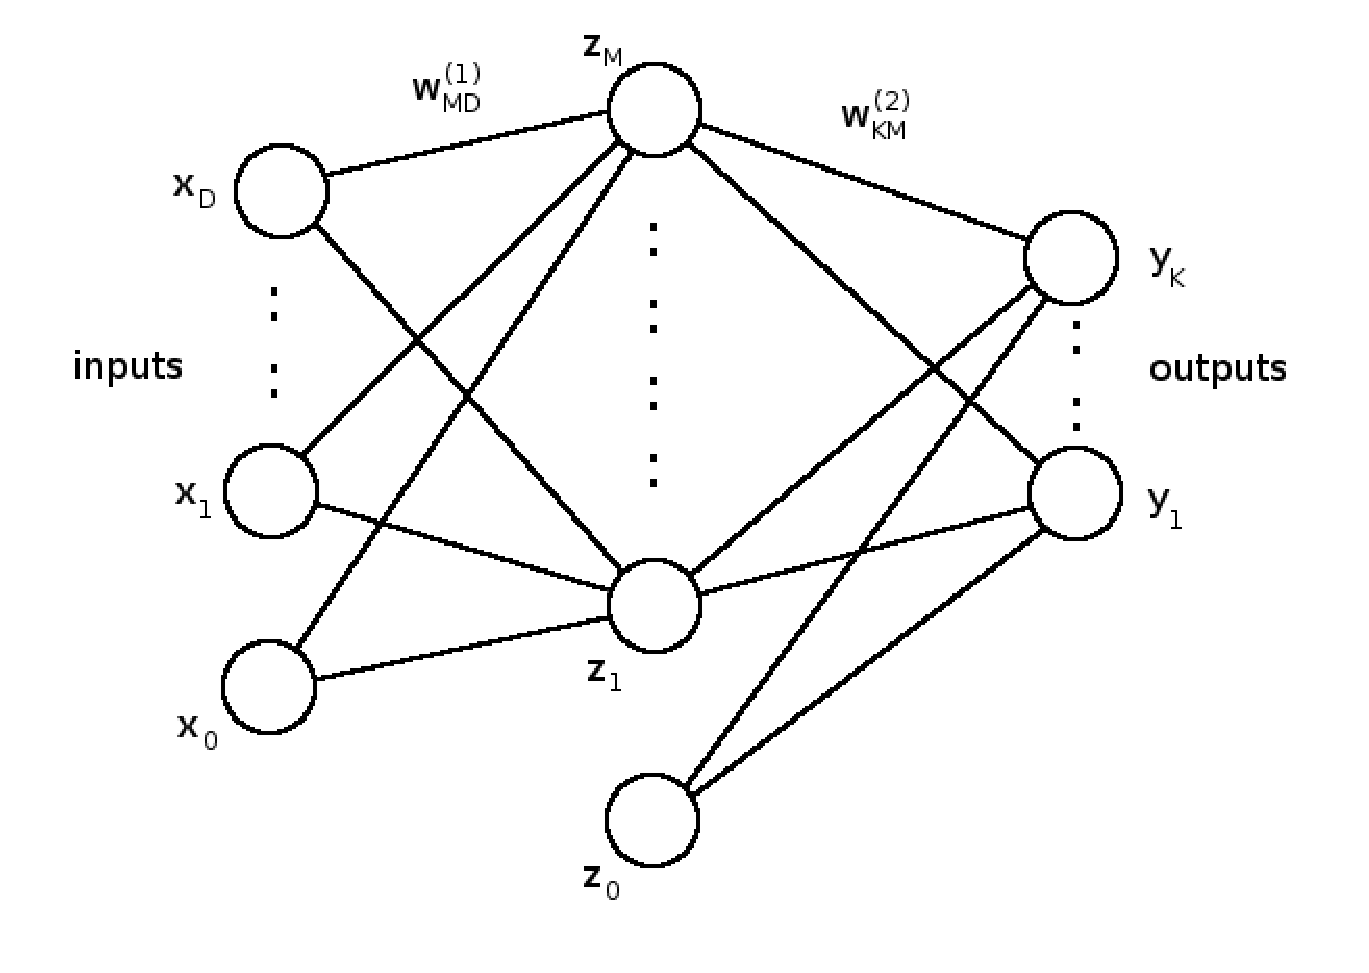
\includegraphics[height=3in]{04ANN/ANNetwork.eps}
\end{center}
\caption{โครงสร้างของโครงข่ายประสาทเทียมแบบจ่ายไปข้างหน้า. {\footnotesize ภาพดัดแปลงจาก\cite{Bishop2006a}}}
\label{fig: ANN feed-forward structure}
\end{figure}
%

\textit{ชั้นอินพุต} (input layer) คือกลุ่มของค่าอินพุตของโครงข่ายและไบอัส เช่น $x_1, \ldots, x_D$ และ $x_0$ ในรูป~\ref{fig: ANN feed-forward structure}.
%ชั้นเอาต์พุต (output layer) คือกลุ่มของหน่วยย่อย ที่เอาต์พุตของหน่วยย่อยเป็นเอาต์พุตของโครงข่าย.
\textit{ชั้นซ่อน} (hidden layer) คือกลุ่มของหน่วยย่อย ที่รับอินพุตมาจากหน่วยย่อยในชั้นก่อนหน้า 
และส่งเอาต์พุตต่อไปให้หน่วยย่อยในชั้นถัดไป เช่น หน่วยย่อยที่มีเอาต์พุตเป็น $z_1, \ldots, z_M$ (และ เพื่อความสะดวก รวมถึง $z_0$ ซึ่งเป็น ไบอัสในชั้นซ่อนด้วย) ในรูป.
\textit{ชั้นเอาต์พุต} (output layer) คือกลุ่มของหน่วยย่อยที่ส่งเอาต์พุตออกไปเป็นเอาต์พุตของโครงข่าย เช่น หน่วยย่อยที่มีเอาต์พุตเป็น $y_1, \ldots, y_K$ ในรูป.
หน่วยย่อยที่อยู่ในชั้นซ่อน จะเรียกว่า \textit{หน่วยซ่อน} (hidden unit).
ในรูป~\ref{fig: ANN feed-forward structure} แสดงชั้นซ่อนแค่ $1$ ชั้น ซึ่งหากต้องการ เราสามารถสร้างโครงข่ายให้มีชั้นซ่อนมากกว่านี้ได้ ซึ่งการใช้ชั้นซ้อนจำนวนมากๆ จะเรียกว่าเป็นโครงข่ายแบบลึก.
ชั้นซ่อนในรูป มีจำนวนหน่วยย่อย $M$ หน่วย ดังนั้นจะมีค่าที่คำนวณออกมา คือ $z_1, \ldots z_M$ และ เช่นเดียวกัน ค่า $z_0$ ถูกกำหนดขึ้นมาเพื่อความสะดวก และ $z_0 = 1$ เสมอ.

ในรูป 
เอาต์พุตของโครงข่าย $\mathbf{y}$ มี $K$ มิติ.
นั่นคือ $\mathbf{y} = [y_1, \ldots, y_K]^T$.
ค่าของเอาต์พุตของหน่วยย่อยแต่ละตัว (ทั้ง $z_1, \ldots, z_M$ และ $y_1, \ldots, y_K$) คำนวณจาก สมการ~\ref{eq: ANN neural output} และ \ref{eq: ANN neural activation}, เช่น
\begin{eqnarray}
\mbox{ชั้นที่ 2} \quad
   y_k &= h_2(a^{(2)}_k) =& h_2 \left( \sum_{m=0}^M w^{(2)}_{km} z_m \right)
\nonumber \\
\mbox{และ ชั้นที่ 1} \quad
   z_m &= h_1(a^{(1)}_m) =& h_1\left( \sum_{d=0}^D w^{(1)}_{md} x_d \right)
   %, \quad \mbox{สำหรับ} \quad m = 1, \ldots, M.
\nonumber
\end{eqnarray}
เมื่อ $h_1(\cdot)$, $h_2(\cdot)$  เป็นฟังชั่นกระตุ้นของชั้นที่ 1 และ 2 ตามลำดับ,
$a^{(1)}_m$, $m=1,\ldots,M$ และ
$a^{(2)}_k$, $k=1,\ldots,K$ เป็น การกระตุ้นของหน่วยย่อยต่างๆของชั้นที่ 1 และ 2 ตามลำดับ.
จากสมการข้างต้น ความสัมพันธ์ระหว่าง เอาต์พุตของโครงข่าย $y_k$ กับ อินพุต $x_d$ คือ
\begin{eqnarray}
   y_k &=& h_2\left( w^{(2)}_{k0} +\sum_{m=1}^M w^{(2)}_{km} \cdot h_1\left( w^{(1)}_{m0} + \sum_{d=1}^D w^{(1)}_{md} x_d \right) \right).
\label{eq: ANN 2-layer output}
\end{eqnarray}
%
เมื่อเปรียบเทียบสมการ~\ref{eq: ANN 2-layer output} กับ \ref{eq: ANN lin model} จะเห็นว่า $z_m$ ทำหน้าที่เหมือนกับค่าเบซิสฟังชั่นในสมการ~\ref{eq: ANN lin model}.
%
เพื่อความสะดวก เราสามารถเขียนสมการ~\ref{eq: ANN neural output} และ \ref{eq: ANN neural activation} ได้ในรูปเมตริกซ์ได้,
\begin{eqnarray}
\mathbf{z}^{(l)} &=& \mathbf{h}(\mathbf{a}^{(l)})
\label{eq: ANN neural output matrix} \\
\mathbf{a}^{(l)} &=& \mathbf{W}^{(l)} \cdot \mathbf{\dot{z}}^{(l-1)}
\label{eq: ANN neural activation matrix} \\
\mathbf{\dot{z}}^{(l-1)} &=& [1, \; z_1^{(l-1)}, \; z_2^{(l-1)}, \; \ldots, \; z_P^{(l-1)}]^T
\label{eq: ANN neural bias inclusion matrix}
\end{eqnarray}
เมื่อ 
การกระตุ้นของหน่วยต่างๆในชั้น $l$ คือ $\mathbf{a}^{(l)} = [a_1^{(l)}, \; a_2^{(l)}, \;\ldots, \;a_Q^{(l)}]^T$, เมื่อชั้น $l$ มี $Q$ หน่วย.
ฟังชั่นกระตุ้น $\mathbf{h}(\cdot)$ ทำงานกับเมตริกซ์แบบตัวต่อตัว
นั่นคือ $\mathbf{h}([a_1^{(l)}, \;\ldots, \;a_Q^{(l)}]^T) = [h(a_1^{(l)}), \;\ldots, \;h(a_Q^{(l)})]^T$.
น้ำหนักของชั้น $l$ คือ $\mathbf{W}^{(l)}$ เป็น เมตริกซ์ขนาด $Q \times (1+P)$
นั่นคือ $\mathbf{W}^{(l)} = [w_{qp}^{(l)}]_{q=1,\ldots,Q;p=0,\ldots,P}$
และ $\mathbf{z}^{(0)} = \mathbf{x}$.
หมายเหตุ เราสามารถกำหนดฟังชั่นการกระตุ้น $\mathbf{h}(\cdot)$ แตกต่างไปสำหรับแต่ละชั้นได้
โดยใช้ตัวแปร  $\mathbf{h}^{(l)}(\cdot)$ แทน เพื่อระบุว่าเป็นฟังชั่นของชั้น $l$.

ในทำนองเดียวกันสำหรับโครงข่าย $2$ ชั้น สมการ~\ref{eq: ANN 2-layer output} สามารถแจกแจงได้เป็น
\begin{eqnarray}
\mathbf{\dot{x}} &=& [1, \; \mathbf{x}]
\label{eq: ANN 2-layer x dot} \\
\mathbf{z} &=& \mathbf{h}( \mathbf{W}^{(1)} \cdot \mathbf{\dot{x}})
\label{eq: ANN 2-layer z} \\
\mathbf{\dot{z}} &=& [1, \; \mathbf{z}]
\label{eq: ANN 2-layer z dot} \\
\mathbf{y} &=& \bm{\sigma}( \mathbf{W}^{(2)} \cdot \mathbf{\dot{z}})
\label{eq: ANN 2-layer output matrix} 
\end{eqnarray}
เมื่อ $\bm{\sigma}(\cdot)$ คือ ฟังชั่นกระตุ้นชั้นเอาต์พุต ที่ทำงานกับเมตริกซ์แบบตัวต่อตัว.
รายการ~\ref{lst: ann nnOutput} แสดงโปรแกรมในภาษาอาร์โปรเจคสำหรับคำนวณค่าเอาต์พุตของโครงข่าย
โดยอาศัยความสามารถเชิงเมตริกซ์ของอาร์โปรเจค.

%\begin{minipage}{5.5in}
{\small
\begin{shaded}
การเขียนโปรแกรมในรูปเมตริกซ์ช่วยให้โปรแกรมกระชับและอ่านง่ายขึ้น.
นอกจากนั้น
สำหรับระบบการคำนวณที่สนับสนุนการคำนวณเมตริกซ์ เช่น อาร์โปรเจค, แมทแลป, และ ไพธอน-นัมไพ.
โปรแกรมที่เขียนโดยใช้คุณสมบัติการคำนวณเมตริกซ์ 
จะให้ผลการรันที่มีประสิทธิภาพมากกว่าโปรแกรมที่ทำงานเดียวกันแต่เขียนโดยใช้การวนลูป
เนื่องจากระบบเหล่านี้ ภายในได้มีการปรับแต่งเพื่อการคำนวณเมตริกซ์อย่างมีประสิทธิภาพมาแล้ว
\end{shaded}
}
%\end{minipage}

\subsection{ฟังชั่นกระตุ้น}
\label{sec: ANN Activation Function}

หัวข้อ~\ref{sec: Multilayer Perceptron} อภิปรายว่า โครงข่ายประสาทเทียมใช้ฟังชั่นซิกมอยด์เป็นฟังชั่นกระตุ้น.
โดยทั่วไป เราสามารถกล่าวได้ว่า ฟังชั่นซิกมอยด์เป็นฟังชั่นกระตุ้นที่เหมาะสมและใช้งานได้ดีกับโครงข่ายประสาทเทียม
ยกเว้นฟังชั่นกระตุ้นของหน่วยย่อยในชั้นเอาต์พุต ที่สำหรับงานบางประเภท ฟังชั่นกระตุ้นชนิดอื่นจะมีความเหมาะสมกับงานมากกว่า.
เพื่อจำแนกความต่าง ให้ $\sigma(\cdot)$ แทนฟังชั่นกระตุ้นของหน่วยย่อยในชั้นเอาต์พุต.
เราสามารถเขียนสมการ~\ref{eq: ANN 2-layer output} สำหรับโครงข่ายจ่ายไปข้างหน้า $2$ ชั้น ได้เป็น
\begin{eqnarray}
   y_k &=& \sigma( a^{(2)}_k )
\label{eq: ANN 2-layer network output} \\
   a^{(2)}_k &=& w^{(2)}_{k0} + \sum_{j=1}^M w^{(2)}_{kj} \cdot z^{(1)}_j
\label{eq: ANN 2-layer activation 2} \\  
   z^{(1)}_j &=& h( a^{(1)}_j )
\label{eq: ANN 2-layer output 1} \\  
   a^{(1)}_j &=& w^{(1)}_{j0} + \sum_{i=1}^D w^{(1)}_{ji} \cdot z^{(0)}_i
\label{eq: ANN 2-layer activation 1} \\     
   z^{(0)}_i &=& x_i
\label{eq: ANN 2-layer network input}
\end{eqnarray}
โดย $h(\cdot)$ เป็นฟังชั่นซิกมอยด์ นั่นคือ $h(a) = 1/\{1 + \exp(a)\}$ 
และฟังชั่นกระตุ้นชั้นเอาต์พุต $\sigma(\cdot)$ 
จะขึ้นกับ ชนิดของงานที่นำโครงข่ายประสาทเทียมไปใช้ (ตาราง~\ref{tbl: ANN output activation function}).

สังเกตุสมการ~\ref{eq: ANN 2-layer network output} และ \ref{eq: ANN 2-layer activation 2} คือ เอาต์พุตและการกระตุ้นของโครงข่ายชั้นที่สอง.
%เนื่องจากโครงข่ายนี้มี $2$ ชั้น เอาต์พุตของชั้นที่สอง ก็เป็นเอาต์พุตของโครงข่ายด้วย.
ในลักษณะเดียวกัน สมการ~\ref{eq: ANN 2-layer output 1} และ \ref{eq: ANN 2-layer activation 1} คือ เอาต์พุตและการกระตุ้นของโครงข่ายชั้นที่หนึ่ง.
สมการ~\ref{eq: ANN 2-layer network input} คือ อินพุตของโครงข่าย หรือ อาจจะมองเป็นเสมือนกับ เอาต์พุตชั้นที่ศูนย์ก็ได้.
ลักษณะเช่นนี้ เป็นดังรูปแบบสมการ~\ref{eq: ANN neural output} และ \ref{eq: ANN neural activation} ที่ถกกันไป.

%
\begin{table}[hbtp]
%{\large
\caption{ฟังชั่นกระตุ้นสำหรับหน่วยย่อยในชั้นเอาต์พุตของโครงข่ายประสาทเทียม
(ดัชนีบนของการกระตุ้นถูกละไว้เพื่อความกระชับของสมการ)}
\begin{center}
\begin{tabular}{|l|}
\hline 
\\
\textit{การหาค่าถดถอย} (regression) ใช้ฟังชั่นเอกลักษณ์ \\
\multicolumn{1}{|c|}{$y_k = a_k$.} \\
\\
\textit{การจำแนกประเภทสองกลุ่ม} (biclass classification) ใช้ฟังชั่นซิกมอยด์ \\
\multicolumn{1}{|c|}{$y_k = \frac{1}{1+\exp(-a_k)}$.} \\
\\
\textit{การจำแนกประเภทหลายกลุ่ม} (multiclass classification) ใช้ฟังชั่นซอฟต์แม็กซ์ \\ 
\multicolumn{1}{|c|}{$y_k = \frac{\exp(a_k)}{\sum_q \exp(a_q)}$.} \\
\\
\hline
\end{tabular} 
\end{center}
\label{tbl: ANN output activation function}
%}%end \large
\end{table}

เราพิจารณาการใช้งานโครงข่ายประสาทเทียม กับ งาน $3$ ชนิดหลักๆ คือ การหาค่าถดถอย, การจำแนกประเภทสองกลุ่ม, และ การจำแนกประเภทหลายกลุ่ม.
การใช้\textit{ฟังชั่นเอกลักษณ์} (identity function: $y_k = a^{(2)}_k$) จะทำงานได้ดีกับงานการหาค่าถดถอย
นั่นคือ เอาต์พุตของโมเดลสามารถมีค่าได้ทุกค่าของจำนวนจริง.
การใช้ฟังช่นเอกลักษณ์จะไม่จำกัดค่าของเอาต์พุตอยู่แค่ในช่วง $0$ ถึง $1$ แบบที่เกิดขึ้นกับการใช้ฟังชั่นซิกมอยด์.
%
งานการจำแนกประเภทสองกลุ่ม เป็นงานชนิดที่ฟังชั่นซิกมอยด์เหมาะที่จะใช้เป็นฟังชั่นกระตุ้น.
%, เราจะใช้ sigmoid function, $y_k = 1/\{1+\exp(a^{(2)}_k)\}$.
สำหรับการจำแนกประเภทสองกลุ่ม ฟังชั่นซิกมอยด์จะทำงานได้ดีกว่าฟังชั่นเอกลักษณ์ ดังเหตุผลที่อธิบายในหัวข้อ~\ref{section: Logistic Regression}.
%, $h_2(\cdot) = h_1(\cdot) = h(\cdot)$ หรือ
%$
%   y_k = h\left(w^{(2)}_{k0} +\sum_{m=1}^M w^{(2)}_{km} h\left( w^{(1)}_{m0} + \sum_{d=1}^D w^{(1)}_{md} x_d \right) \right)
%$
%เมื่อ $y_k$ คือ เอาต์พุตที่ $k$.
นอกจากนั้น การใช้ฟังชั่นซิกมอยด์ยังทำให้เราสามารถตีความค่าเอาต์พุต $y_k$ ในเชิงความน่าจะเป็นได้.
เช่น ค่าเอาต์พุตอาจตีความเป็นค่าทำนายความน่าจะเป็นที่จะจัดเป็นกลุ่ม 1 กรณีที่แบ่งระหว่างกลุ่ม 0 กับ กลุ่ม 1.
ถ้าค่า $y_k$ ใกล้กับ $1$ ก็หมายความว่า มีความน่าจะเป็นของกลุ่ม 1 สูง
การทายกลุ่ม 1 จึงสมเหตุสมผล.
.
แต่ถ้าค่า $y_k$ ใกล้กับ $0$ ก็หมายความว่า มีความน่าจะเป็นของกลุ่ม 0 ซึ่งคือ $1 - y_k$ มีค่าสูง
ดังนั้นหากทายกลุ่ม 0 ก็จะมีโอกาสถูกมากกว่า.
%
การจำแนกประเภทแบบหลายกลุ่ม เราสามารถใช้รหัสหนึ่งไปเค (1-of-K coding) และใช้ฟังชั่นกระตุ้นเป็น\textit{ฟังชั่นซอฟต์แมกซ์} (softmax function) \index{ซอฟต์แมกซ์} \index{softmax function} เช่นเดียวกับที่ถกในหัวข้อ~\ref{section: multiclass classification}.
% , คือ จะกำหนดให้เอาต์พุตมี $K$ มิติ, ซึ่ง เท่ากับจำนวนกลุ่มที่จะแบ่ง.
ฟังชั่นซอฟต์แมกซ์ $y_k = \frac{\exp(a^{(2)}_k)}{\sum_{q=1}^K \exp(a^{(2)}_q)}$ ก็สามารถมองเป็นการตีความเอาต์พุต $y_k$ ในเชิงความน่าจะเป็นได้ เช่นกัน.
นั่นคือ $y_k$ แทนค่าทำนายความน่าจะเป็นที่จะเป็นกลุ่ม k.
สังเกตุว่า $0 \leq y_k \leq 1$ และ $\sum_k y_k = 1$ ซึ่งไม่ได้ละเมิดคุณสมบัติของความน่าจะเป็น.
ตาราง~\ref{tbl: ANN output activation function} สรุปฟังชั่นกระตุ้นของชั้นเอาต์พุต สำหรับงานหลักๆของการประยุกต์ใช้โครงข่ายประสาทเทียม.

{\small
\begin{shaded}
\paragraph{\small เกร็ดความรู้เซลล์ประสาท}
(เรียบเรียงจาก \cite{BuddhasBrain} และ \cite{Wikipedia})
\index{เซลล์ประสาท}\index{Biological Neurons}
%\footnote{จาก \url{https://en.wikipedia.org/wiki/Brain_size} (สืบค้น 21 ส.ค. 2559)}
สมองมนุษย์ประกอบเซลล์ชนิดต่างๆมากมาย
เช่น 
เส้นเลือด 
เซลล์เกลีย
เซลล์ประสาท.
เส้นเลือดทำหน้าที่รับส่งอากาศ น้ำ อาหาร.
\textit{เซลล์เกลีย}(neuroglia) ทำหน้าที่สนับสนุนต่างๆ รวมถึงการรักษา\textit{ภาวะธำรงดุล} (homeostasis) เพื่อให้ภายในสมองมีสภาวะที่เหมาะ เช่น การควบคุมระดับความเข้มข้นของโซเดียมและแคลเซียมไอออน เป็นต้น.
%ซึ่งในจำนวนนั้น 
เซลล์ประสาททำหน้าที่หลักของสมอง ได้แก่การควบคุมระบบการทำงานต่างๆในร่างกายให้เป็นปกติ 
รวมไปถึง การให้ความสามารถในการจำ การเรียนรู้ การคิด และการทำความเข้าใจ.

สมองมนุษย์มีเซลล์ประสาทอยู่ประมาณแสนล้านเซลล์ 
เซลล์ประสาทเองก็มีอยู่หลายประเภท แต่โครงสร้างพื้นฐานมีลักษณะคล้ายๆกัน
%
นั่นคือเซลล์ประสาทแต่ละเซลล์มีใยประสาทเพื่อรับสัญญาณเข้าสู่เซลล์เรียกว่า\textit{เดนไดรต์}(dendrite).
สัญญาณต่างๆที่เข้าสู่เซลล์จะถูกนำมารวมกันที่นิวเคลียส
และผลรวมของสัญญาณที่รับเข้ามา ทั้งสัญญาณกระตุ้นและสัญญาณยับยั้ง 
จะเป็นตัวตัดสินว่าเซลล์ประสาทนั้นจะอยู่ในสถานะถูกกระตุ้นหรือไม่.
ถ้าเซลล์ประสาทอยู่ในสถานะถูกกระตุ้น มันจะส่งสัญญาณออกไปให้กับเซลล์ประสาทอื่นๆที่รับสัญญาณจากมัน
ผ่านใยประสาทนำออกสัญญาณเรียกว่า\textit{แอกซอน}(axon). 
จุดต่อระหว่างแอกซอนของเซลล์ประสาทตัวหนึ่งกับเดนไดรต์ของเซลล์ประสาทอีกเซลล์หนึ่ง 
%เซลล์ประสาทแต่ละเซลล์เชื่อมต่อกับเซลล์ประสาทอื่นๆผ่าน
เป็นจุดประสานประสาทที่เรียกว่า \textit{ไซแนปส์} (synapse).
แนวคิดพื้นฐานนี้เองที่ โรเซนแบลท นำไปสร้างโมเดลเพอร์เซปตรอน (ดูรูป~\ref{fig: ANN neuron} และ \ref{fig: ANN synapse} ประกอบ)
เมื่อเปรียบเทียบเพอร์เซปตรอนกับเซลล์ประสาท ผลคูณของอินพุตกับค่าน้ำหนักของเพอร์เซปตรอน (เช่น \verb|x[D]| กับ \verb|w[D]| ในรูป~\ref{fig: ANN perceptron}) เทียบได้กับ ความแรงของสัญญาณประสาทสัญญาณหนึ่งที่รับเข้ามาผ่านไซแนปส์แล้วกำลังเดินทางเข้าสู่นิวเคลียสของเซลล์ประสาท
เพื่อไปรวมกับความแรงของสัญญาณประสาทสัญญาณอื่นๆที่รับเข้ามาผ่านไซแนปส์จุดอื่นๆ.
ความแรงของสัญญาณประสาทสัญญาณหนึ่งที่รับเข้ามาผ่านไซแนปส์ จะขึ้นอยู่กับ
สัญญาณที่ส่งมา (เปรียบเทียบกับ \verb|x[D]|) และ ความแข็งแรงในการเชื่อมต่อสัญญาณของไซแนปส์ (เปรียบเทียบกับ \verb|w[D]|).

โดยเฉลี่ยแล้ว เซลล์ประสาทแต่ละเซลล์จะมีไซแนปส์ประมาณห้าพันจุด
ซึ่งนั่นคือเมื่อรวมแล้ว ในสมองมนุษย์หนึ่งคนจะมีการเชื่อมต่อประสาทอยู่ราวๆห้าร้อยล้านล้านไซแนปส์.
การรับส่งสัญญาณประสาทระหว่างเซลล์ประสาทมีหลายกลไก เช่น กลไกทางเคมี (ผ่านสารสื่อประสาท) กลไกทางไฟฟ้า และ กลไกเชิงภูมิคุ้มกัน.
แต่กลไกหลักของการส่งสัญญาณประสาทคือกลไกทางเคมี
ซึ่งคือการรับส่งสัญญาณประสาทระหว่างเซลล์ประสาทโดยดำเนินการผ่าน\textit{สารสื่อประสาท} (neurotransmitter). 
เซลล์ประสาทที่ส่งสัญญาณจะปล่อยสารสื่อประสาทออกมาผ่านโปรตีนที่ทำหน้าที่ส่งสารสื่อประสาท เรียกว่า \textit{ทรานสปอร์ตเตอร์} (neurotransmitter transporter) 
และเซลล์ประสาทที่รับสัญญาณจะรับสารสื่อประสาทเหล่านั้นเข้าไปผ่านโปรตีนที่ทำหน้าที่รับสารสื่อประสาท เรียกว่า \textit{รีเซปเตอร์} (receptor).
% 220 MPH speed of neural impulse\cite{GodwinCham2012a}


%[กลไกของ chemical synapse: binding to response]
เมื่อรีเซปเตอร์รับสารสื่อประสาทเข้ามา
นั่นคือ โครงสร้างของสารสื่อประสาทจับกับโครงสร้างของรีเซปเตอร์
แล้วทำให้กลไกของรีเซปเตอร์เปิดทำงาน
%เพื่อรับโมเลกุลของสารสื่อประสาทเข้าสู่เซลล์ประสาท.
%
โมเลกุลที่จับกับรีเซปเตอร์ จะเรียกว่า \textit{ลิแกนต์} (ligand).
กลไกของการจับตัวระหว่างรีเซปเตอร์กับลิแกนต์นี้
จะเป็นกลไกในลักษณะแม่กุญแจ-ลูกกุญแจ.
นั่นคือ โครงสร้างของรีเซปเตอร์แต่ละชนิดจะจับตัวได้เฉพาะกับลิแกนต์ที่มีโครงสร้างที่เข้ากันได้เท่านั้น
เช่น สารสื่อประสาท\textit{อาเซ็ตทิลคอลีน} (acetylcholine) ซึ่งเป็นสารสื่อประสาทที่เซลล์ประสาทใช้ติดต่อกระตุ้นเซลล์กล้ามเนื้อ
จะจับกับรีเซปเตอร์สำหรับอาเซ็ตทิลคอลีนได้เท่านั้น
และ รีเซปเตอร์สำหรับสารสื่อประสาทตัวอื่น ก็ไม่อาจจับกับอาเซ็ตทิลคอลีนได้เช่นกัน.
การเข้าใจกลไกการทำงานลักษณะนี้ 
ช่วยให้เภสัชศาสตร์สามารถออกแบบตัวยาที่เฉพาะเจาะจงกับสารสื่อประสาทเฉพาะตัวได้
เช่น ยาต้านอาการเศร้าซึม \textit{ฟลูโอเซตทีน} (Fluoxetine) ที่เฉพาะเจาะจงกับสารสื่อประสาท\textit{เซอโรโทนิน}(Serotonin).

หมายเหตุ เซลล์ประสาทแต่ละชนิดจะมีลักษณะเฉพาะตัวต่างกันและจะทำงานกับสารสื่อประสาทเฉพาะชนิด
เช่น
\textit{เซลล์ประสาทเซอโรโทนิน} (serotonin neurons) ที่อยู่บริเวณ\textit{ดอร์ซอลราฟีนูเคลียส} (dorsal raphe nucleus) ของก้านสมอง จะทำงานกับสารสื่อประสาทเซอโรโทนิน\cite{LiEtAl2016a},
\textit{เซลล์ประสาทซีเอ1พีรามิดอล} (CA1 pyramidal neurons) ที่อยู่บริเวณ\textit{ซีเอ1} (CA1) ของฮิปโปแคมปัส
จะทำงานกับสารสื่อประสาท\textit{กลูตาเมท}(Glutamate)\cite{NeuroBank},
\textit{เซลล์ประสาทมิดเบรนโดพามิเนอจิก} (midbrain dopaminergic neurons) ที่อยู่หลายๆบริเวณรวมถึง \textit{พื้นที่เวนทรอลเทกเมนทอล} (ventral tegmental area) ในสมองส่วนกลาง
จะทำงานกับสารสื่อประสาท\textit{โดพามีน}(Dopamine)\cite{NeuroBank}.
เซลล์ประสาทบางชนิดทำงานกับสารสื่อประสาทมากกว่าหนึ่งชนิด เช่น
เซลล์ประสาทหนามกลาง (medium spiny neurons) ที่อยู่บริเวณบาซอลแกงเกลีย
ส่งสัญญาณออกผ่าน\textit{กาบา} (GABA) แต่สามารถรับสัญญาณผ่านสารสื่อประสาทหลายชนิดรวมถึงกลูตาเมทและโดพามีน.

%$\Box$
\end{shaded}
}

%
\begin{figure}
\begin{center}
\begin{tabular}{cc}
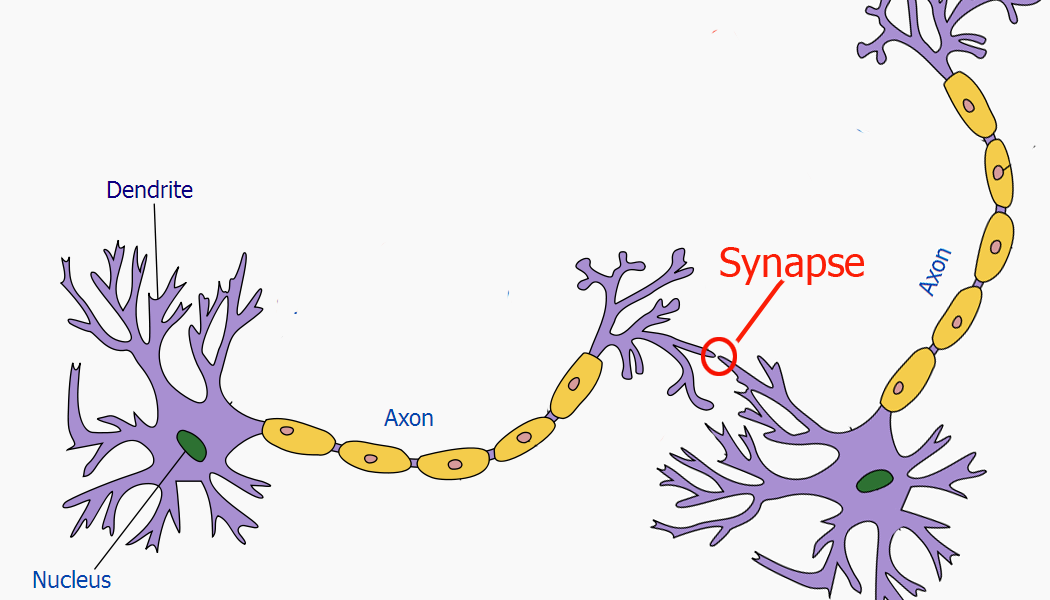
\includegraphics[height=1.8in]{04ANN/Synapse.png}
&
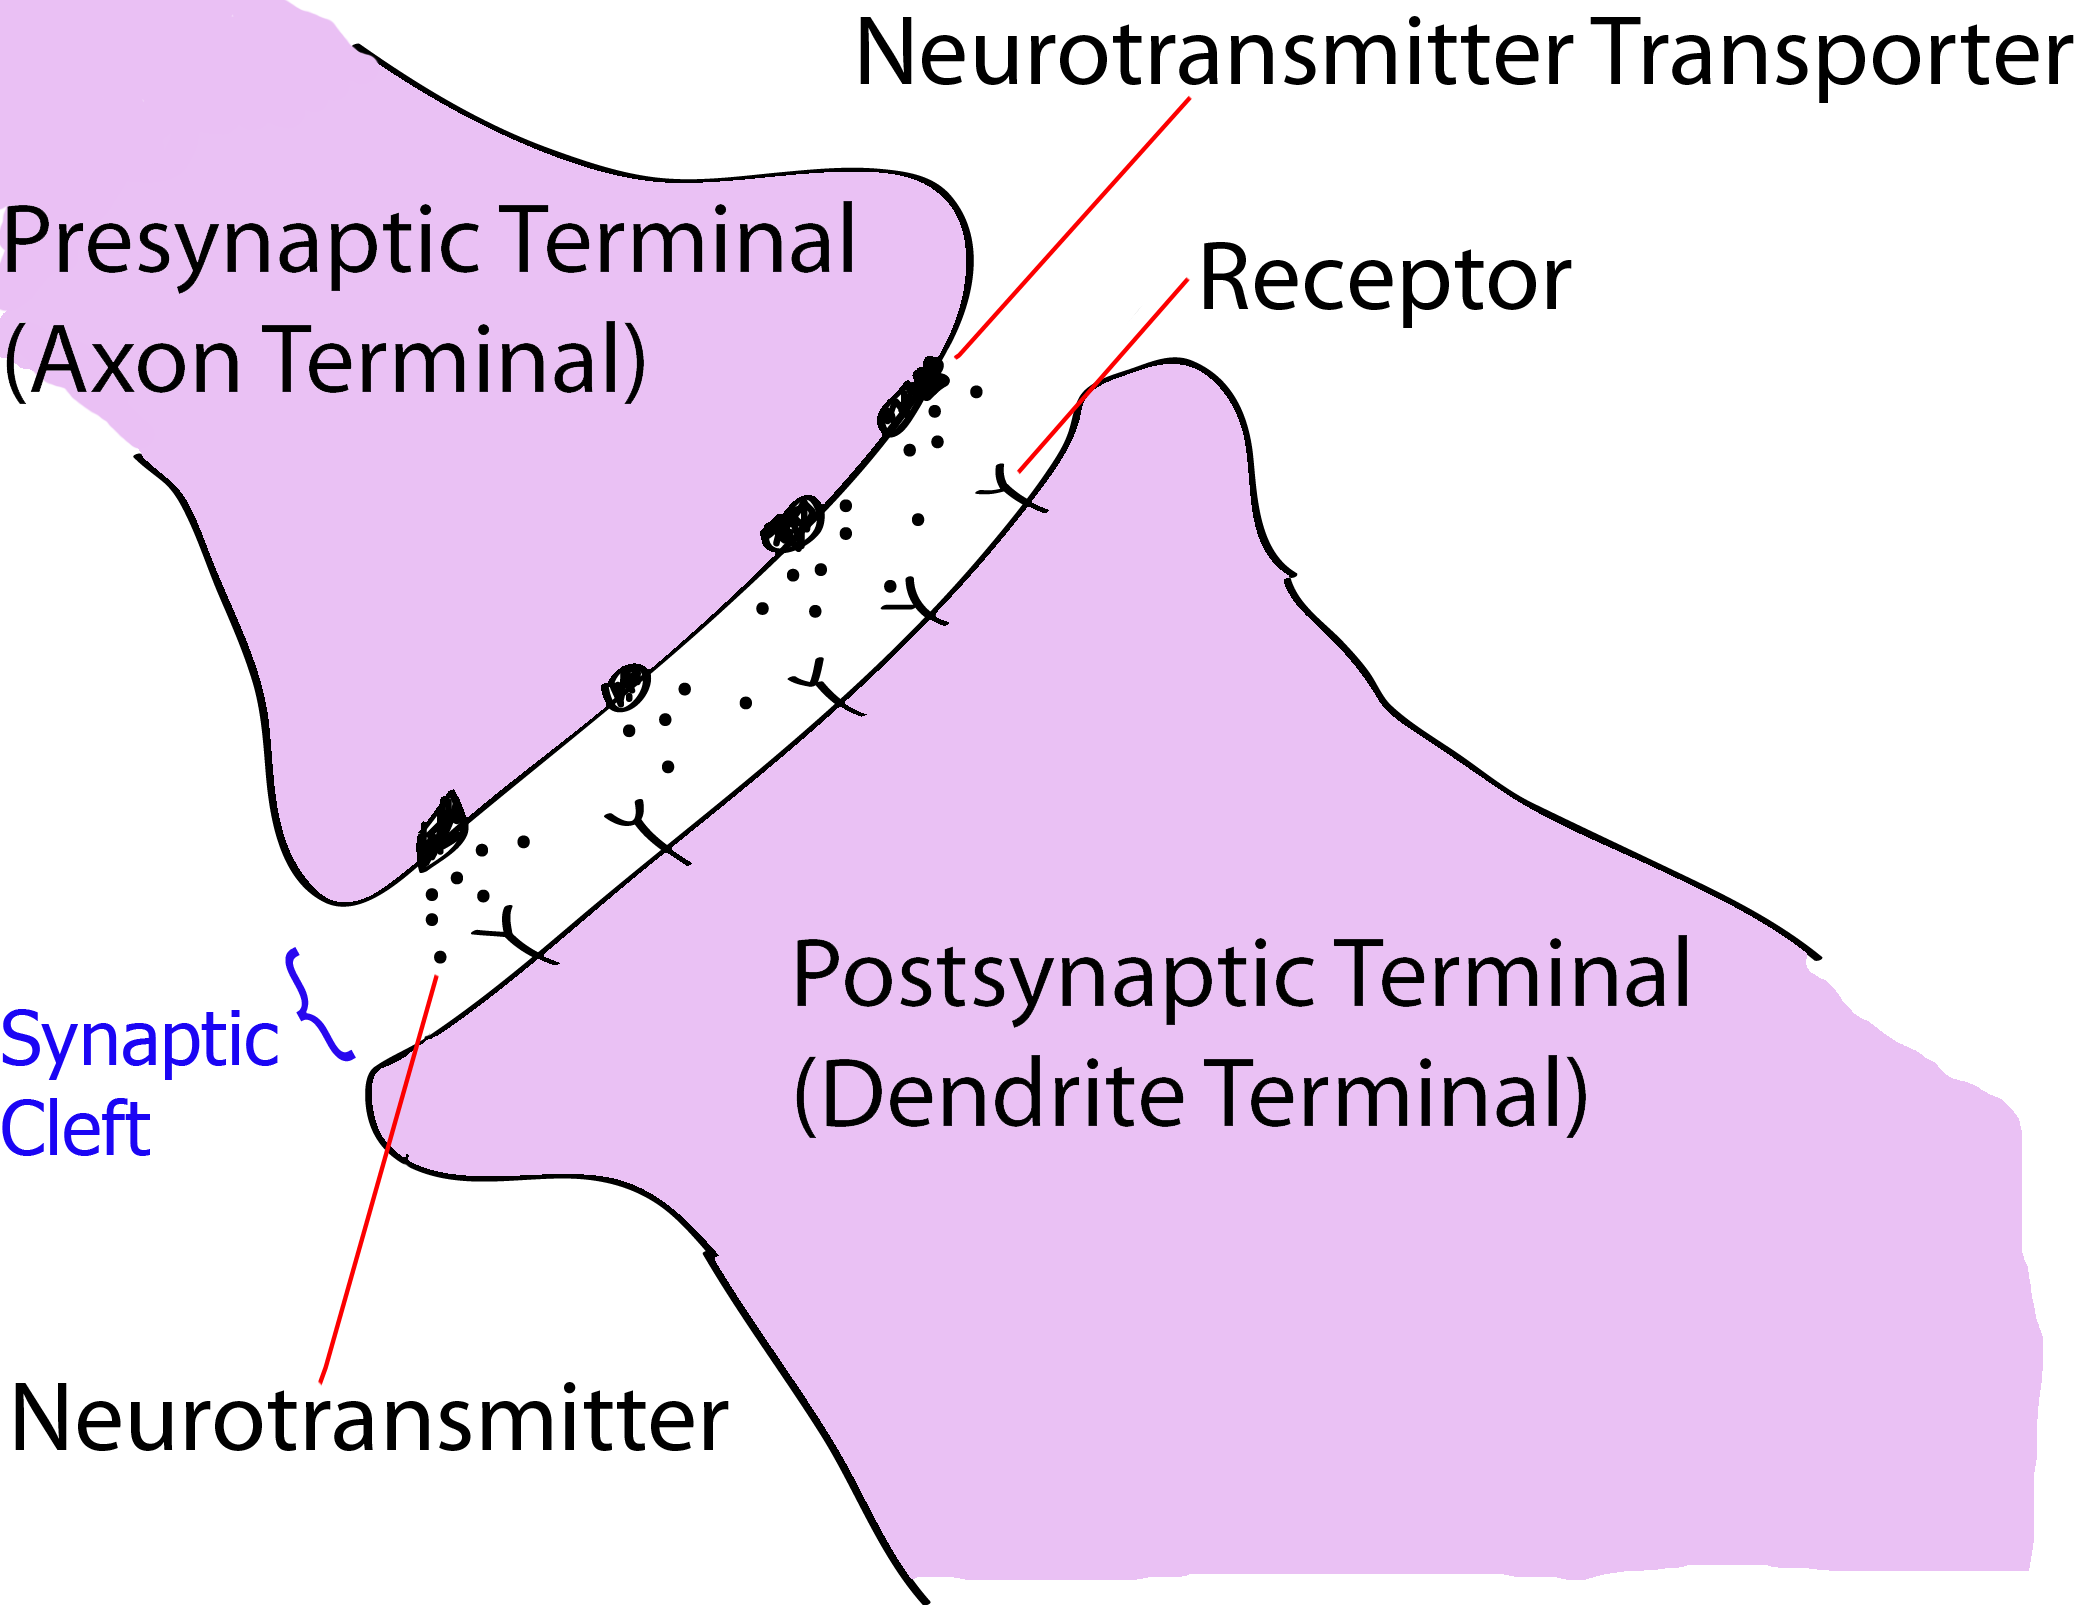
\includegraphics[height=1.8in]{04ANN/chemicalSynapseCol.png}
\\
(ก) & (ข) \\
\end{tabular} 

\end{center}
\caption{ภาพแสดงเซลล์ประสาทเชื่อมต่อสัญญาณกันผ่าน\textit{ไซแนปซ์} (synapse)
โดยสัญญาณที่สื่อสารกันนั้นทำโดยผ่านกลไกของ\textit{สารสื่อประสาท}(neurotransmitter)
(ก) เซลล์ทางซ้ายมือส่งสัญญาณผ่านแอกซอน เชื่อมเข้าสู่อีกเซลล์ที่ไซแนปซ์ เพื่อผ่านเดนไดรต์ไปสู่นิวเคลียสของเซลล์ทางขวามือ
{\footnotesize 
(ภาพดัดแปลงจาก \texttt{http://en.wikipedia.org/wiki/File:Neuron\_Hand-tuned.svg})
}
(ข) ภาพขยายส่วนของไซแนปส์ ซึ่ง\textit{ส่วนปลายของแอกซอน} (presynaptic terminal) จะส่งสารสื่อประสาทออกมา และ\textit{ส่วนปลายของเดนไดรต์} (postsynaptic terminal) จะรับสารสื่อประสาทเข้าไป
}
\label{fig: ANN synapse}
\end{figure}
%





\section{การฝึกโครงข่าย}
\label{sec: ANN training}

เมื่อเรามีโครงข่ายประสาทเทียมแล้ว สิ่งสำคัญที่จะทำให้โครงข่ายสามารถทำงานตามที่เราต้องการได้ก็คือ การใช้ค่าพารามิเตอร์ที่เหมาะสม.
สำหรับโครงข่ายประสาทเทียม, เราจะเรียกการหาค่าพารามิเตอร์หรือค่าน้ำหนักที่เหมาะสมว่า \textit{การฝึกโครงข่าย} (network training).
เราจะฝึกโครงข่าย ด้วยข้อมูลตัวอย่าง ซึ่งประกอบด้วย อินพุตและเอาต์พุตตัวอย่าง $N$ จุดข้อมูล $\{\mathbf{x}_n\}$, $\{\mathbf{t}_n\}$, $n = 1, \ldots, N$ ตามลำดับ.
สิ่งที่เราต้องการคือ ทำนายค่าเอาต์พุต $\mathbf{y}$ จากอินพุตตัวอย่าง $\mathbf{x}_n$ ให้ค่าใกล้เคียงกับ เอาต์พุตตัวอย่าง $\mathbf{t}_n$ มากที่สุด หรือ พูดอีกอย่างคือ ถ้าเราทำการหาค่าถดถอย การฝึกโครงข่าย ก็คือ การหาค่าน้ำหนัก $\bm{\theta} = \{\mathbf{W}^{(1)}, \ldots, \mathbf{W}^{(L)} \}$ (เมื่อ $L$ คือจำนวนชั้นของโครงข่าย) ที่ทำให้ฟังชั่นความผิดพลาดมีค่าน้อยที่สุด.
นั่นคือ $\bm{\theta}^{\ast} = \arg \min_{\bm{\theta}} E(\bm{\theta})$ เมื่อ
\begin{eqnarray}
   E(\bm{\theta}) &=& \frac{1}{2} \sum_{n=1}^N \Vert \mathbf{y}(\mathbf{x}_n, \bm{\theta}) - \mathbf{t}_n \Vert^2
\label{eq: ANN error function}
\end{eqnarray}

ซึ่งเมื่อแทนฟังชั่นของโมเดลที่ใช้เข้าไป เราก็สามารถใช้ วิธีการหาค่าน้อยที่สุด ในการหาค่าน้ำหนัก $\bm{\theta}$ ได้.
ตัวอย่างเช่น หากเราใช้โครงข่ายจ่ายไปข้างหน้า ขนาด $2$ ชั้น,
โมเดลก็คือ
\[
   y_k = w^{(2)}_{k0} +\sum_{m=1}^M w^{(2)}_{km} \cdot h\left( w^{(1)}_{m0} + \sum_{d=1}^D w^{(1)}_{md} x_d \right).
\]

เพื่อความสะดวก เราจะพิจารณา ค่าผิดพลาดที่จุดข้อมูลที่ $n$ เพียงจุดเดียวก่อน, เราจะได้
\begin{eqnarray}
   E_n &=& \frac{1}{2} \sum_{k=1}^K \left\{ y_k - t_{k,n} \right\}^2
\label{eq: ANN En regression} \\   
   &=& \frac{1}{2} \sum_{k=1}^K \left\{ w^{(2)}_{k0} +\sum_{m=1}^M w^{(2)}_{km} \cdot h\left( w^{(1)}_{m0} + \sum_{d=1}^D w^{(1)}_{md} x_{d,n} \right) - t_{k,n} \right\}^2
   \nonumber \\
\label{eq: ANN En 2-layer regression}
\end{eqnarray}
เมื่อ $x_{d,n}$ และ $t_{k,n}$ คือ อินพุตมิติที่ $d$ และ เอาต์พุตมิติที่ $k$ ของจุดข้อมูลที่ $n$ ตามลำดับ.

ดังนั้นค่าอนุพันธ์ของค่าผิดพลาด เมื่อเทียบกับค่าน้ำหนักชั้นที่ 2 คือ
\begin{eqnarray}
   \frac{\partial E_n}{\partial w^{(2)}_{j0}} &=& y_{j,n} - t_{j,n}
\label{eq: ANN dEn/w2 0} \\   
   \frac{\partial E_n}{\partial w^{(2)}_{ji}} &=& (y_{j,n} - t_{j,n}) \cdot z_i^{(1)}, \quad \mbox{เมื่อ} \quad i = 1,\ldots,M
\label{eq: ANN dEn/w2 i}
\end{eqnarray}
และ $z_i^{(1)} = h\left( w^{(1)}_{i0} + \sum_{d=1}^D w^{(1)}_{id} x_{d,n} \right)$.

ในลักษณะเดียวกัน ค่าอนุพันธ์ของค่าผิดพลาดเมื่อเทียบกับค่าน้ำหนักชั้นที่ 1 คือ
\begin{eqnarray}
   \frac{\partial E_n}{\partial w^{(1)}_{ji}} &=& \sum_{k=1}^ K (y_{k,n} - t_{k,n}) \cdot \frac{\partial y_{k,n}}{\partial w^{(1)}_{ji}}
\label{eq: ANN dEn/w1 step 1} \\
   &=& \sum_{k=1}^ K (y_{k,n} - t_{k,n}) \cdot w^{(2)}_{kj} \cdot \frac{\partial h\left( w^{(1)}_{j0} + \sum_{i=1}^D w^{(1)}_{ji} x_{i,n} \right)}{\partial w^{(1)}_{ji}}   
\label{eq: ANN dEn/w1 step 2} \\
   &=& h' ( a_j^{(1)} )  
   \frac{\partial a_j^{(1)} }{\partial w^{(1)}_{ji}} \cdot  \sum_{k=1}^ K (y_{k,n} - t_{k,n}) \cdot w^{(2)}_{kj}    
\label{eq: ANN dEn/w1 step 3}   
\end{eqnarray}
เมื่อ $a_j^{(1)} = w^{(1)}_{j0} + \sum_{i=1}^D w^{(1)}_{ji} x_{i,n}$ และ $h'(a)$ คือ อนุพันธ์ของ $h(a)$.
สำหรับ $h(a) = \frac{1}{1 + \exp(-a)}$, อนุพันธ์ $h'(a) = h(a) \cdot (1 - h(a))$.

ซึ่งสุดท้าย เราจะได้
\begin{eqnarray}
   \frac{\partial E_n}{\partial w^{(1)}_{j0}} &=& h' ( a_j^{(1)} )  
   \cdot  \sum_{k=1}^ K (y_{k,n} - t_{k,n}) \cdot w^{(2)}_{kj}
\label{eq: ANN dEn/w1 0} \\
   \frac{\partial E_n}{\partial w^{(1)}_{ji}} &=& h' ( a_j^{(1)} ) \cdot x_{i,n}  
   \cdot  \sum_{k=1}^ K (y_{k,n} - t_{k,n}) \cdot w^{(2)}_{kj}
   \quad \mbox{เมื่อ} \quad i = 1, \ldots, D.
\nonumber\\   
\label{eq: ANN dEn/w1 i}
\end{eqnarray}

จากสมการ~\ref{eq: ANN dEn/w2 0},~\ref{eq: ANN dEn/w2 i},~\ref{eq: ANN dEn/w1 0},~and~\ref{eq: ANN dEn/w1 i}, ค่าเราสามารถใช้ความรู้จากศาสตร์การหาค่าดีที่สุด เช่น วิธีลงชันที่สุด (รายการ~\ref{lst: steepest descent}) ในการปรับปรุงค่าน้ำหนักได้,
\begin{eqnarray}
   w^{(l)}_{ji}  \gets w^{(l)}_{ji} - \alpha \cdot \frac{\partial E_n}{\partial w^{(l)}_{ji}}
\label{eq: ANN update w grad desc}
\end{eqnarray}
%
โดย ค่าของน้ำหนักใหม่ (เทอมทางซ้ายมือ) จะคำนวณจากค่าน้ำหนักเดิม (เทอมแรกทางขวามือ) ลบค่าอนุพันธ์ของเป้าหมาย ที่คูณด้วย $\alpha$ ที่ทำหน้าที่เป็น\textit{ขั้นก้าว}(step size) หรือ เรียกว่า \textit{อัตราการเรียนรู้} (learning rate) เพื่อรักษาให้อัลกอริทึ่มลู่เข้า, ดังที่ได้ถกในหัวข้อ~\ref{section: Optimization}.

ตัวอย่างและฟังชั่นความผิดพลาด $E(\bm{\theta})$ ที่เราถกกันในหัวข้อนี้ เหมาะกับงานการหาค่าถดถอย.
ดังที่ได้อภิปรายในบท~\ref{chapter: Linear Models} ว่า สำหรับงานการจำแนกประเภท $2$ กลุ่ม การใช้\textit{ฟังชั่นความผิดพลาด} (error function หรือ อาจเรียกว่า \textit{ฟังชั่นเป้าหมาย} objective function หรือ \textit{ฟังชั่นค่าใช้จ่าย} cost function) 
\begin{eqnarray}
   E_n = - t_n \log (y) - (1-t_n) \log(1-y)
\label{eq: ann cost fn biclass}
\end{eqnarray}
จะช่วยให้โมเดลทำงานได้ดีกว่า.
%และ 
สำหรับงานการจำแนกประเภทแบบหลายกลุ่ม เราจะใช้การใช้ฟังชั่นความผิดพลาด 
\begin{eqnarray}
   E_n = - \sum_k t_{kn} \log (y_k).
\label{eq: ann cost fn multiclass}
\end{eqnarray}

\paragraph{การฝึกแบบออนไลน์กับแบบออฟไลน์} 
% online v.s. offline
การฝึกโครงข่ายโดยปรับปรุงค่าน้ำหนัก โดยทำการคำนวณจากจุดข้อมูลทีละจุด (เช่น สมการ~\ref{eq: ANN update w grad desc}) จะเรียกว่า เป็น\textit{การฝึกแบบออนไลน์} (online training) หรือ \textit{การฝึกแบบส่วนเพิ่ม} (incremental mode).
นอกจากการฝึกแบบออนไลน์แล้ว
เราสามารถที่จะรวมผลค่าอนุพันธ์สำหรับทุกๆจุดข้อมูล แล้วปรับปรุงค่าน้ำหนักทีเดียวได้,
\begin{eqnarray}
   w^{(l)}_{ji}  \gets w^{(l)}_{ji} - \alpha \cdot \sum_{n=1}^N \frac{\partial E_n}{\partial w^{(l)}_{ji}}
\label{eq: ANN update w grad desc}
\end{eqnarray}
เมื่อ $N$ คือ จำนวนจุดข้อมูล.
เราจะเรียกการฝึกแบบนี้ว่า \textit{การฝึกแบบออฟไลน์} (offline training) หรือ \textit{การฝึกแบบกลุ่ม} (batch mode).

{\small
\begin{shaded}
ในทางปฏิบัติ 
ลำดับของข้อมูลจะถูกสลับในแต่ละรอบฝึกทั้งในการฝึกแบบออฟไลน์และออนไลน์
เพื่อคุณภาพของการฝึกที่ดี (ลดความเสี่ยงที่น้ำหนักจะไปติดกับค่าที่ไม่ดีตั้งแต่แรกและจะปรับเปลี่ยนยากในภายหลัง).

การเลือกระหว่างการฝึกแบบออนไลน์กับแบบออฟไลน์
เฮย์กิน\cite{Haykin2009a}ได้อภิปรายถึงข้อดีข้อเสียดังนี้.
การฝึกแบบออฟไลน์จะให้การประมาณค่าเกรเดียนต์ที่แม่นยำ ดังนั้นจึงรับประกันว่าเมื่อทำงานกับวิธีลงเกรเดียนต์แล้วจะได้น้ำหนักที่เป็นค่าตัวทำน้อยที่สุด(ท้องถิ่น).
นอกจากนั้น การฝึกแบบออฟไลน์ยังเป็นการคำนวณแบบขนาน (และสามารถนำศาสตร์และเทคโนโลยีการประมวลผลแบบขนานมาช่วยได้)
และ เมื่อมองจากมุมมองทางสถิติศาสตร์ การฝึกแบบออฟไลน์ก็เป็นรูปแบบ\textit{การอนุมานทางสถิติ}(statistical inference)อย่างหนึ่ง 
ดังนั้นการฝึกแบบออฟไลน์จะเหมาะกับงานการหาค่าถดถอย.
แต่ข้อเสียของการฝึกแบบออฟไลน์ ก็คือความต้องการใช้หน่วยความจำปริมาณมาก (เพราะว่าใช้ข้อมูลทั้งหมด ในการคำนวณแต่ละยก).

ข้อดีของการฝึกแบบออนไลน์เมื่อทำร่วมกับการสลับลำดับของข้อมูลแต่ละรอบฝึกจะช่วยลดความเสี่ยงในการเข้าไปติดอยู่ในค่าตัวทำต่ำสุดท้องถิ่นได้
และเมื่อเทียบกับการฝึกแบบออฟไลน์ การฝึกแบบออนไลน์จะต้องการใช้หน่วยความจำปริมาณน้อยกว่า.
นอกจากนั้นในทางปฎิบัติแล้วพบว่า การฝึกแบบออนไลน์จะสามารถใช้ประโยชน์จากข้อมูลที่ซ้ำซ้อนกันได้มากกว่าการฝึกแบบออฟไลน์
และการฝึกแบบออนไลน์ยังช่วยให้เราสามารถติดตามการเปลี่ยนแปลงเล็กๆในข้อมูลได้ด้วย โดยเฉพาะอย่างยิ่งเมื่อกระบวนการที่อยู่เบื้องหลังข้อมูล (กระบวนการที่สร้างข้อมูล) เป็นกระบวนการที่\textit{ไม่นิ่งทางสถิติ} (nonstationary).
แม้ว่าการฝึกแบบออนไลน์จะทำงานได้ช้ากว่า
แต่การฝึกแบบออนไลน์ก็มีการใช้อย่างแพร่หลายโดยเฉพาะกับ\textit{งานการจำแนกรูปแบบ} (pattern-classification task)
เพราะว่า การฝึกแบบออนไลน์นั้นนำไปสร้างหรือเขียนโปรแกรมได้ง่ายกว่า
และ สามารถขยายขึ้นไปทำงานกับข้อมูลขนาดใหญ่และใช้กับปัญหาการจำแนกรูปแบบยากๆได้.
\end{shaded}
}%

\paragraph{\textit{รอบฝึก} (epoch)} 
เนื่องจากวิธีการฝึกจะเป็นการคำนวณซ้ำหลายๆรอบ.
เราจะเรียก การปรับปรุงค่าน้ำหนักครบทุกตัวในแต่ละยกว่าเป็น $1$ \textit{รอบฝึก} (epoch).
โดยทั่วไป แล้วเราต้องทำการฝึกหลายรอบ ก่อนที่ค่าน้ำหนักจะลู่เข้าหาค่าทำต่ำสุด.
จำนวนรอบฝึกที่ต้องทำขึ้นกับหลายปัจจัย เช่น ความซับซ้อนของปัญหา, ขนาดและความซับซ้อนของโครงข่าย, อัตราการเรียนรู้, ค่าเริ่มต้น, และ วิธีการที่ใช้ฝึก.
ดูหัวข้อ~\ref{sec: ANN suggestions} เพิ่มเติม สำหรับคำแนะนำวิธีการเลือกจำนวนรอบฝึก.



\section{การแพร่กระจายย้อนกลับ}
\label{sec: ANN backpropagation}

เราได้เห็นภาพรวมของการฝึกโครงข่ายแล้ว %และ จากหัวข้อ~\ref{sec: ANN training}.
ซึ่งหัวใจของการฝึกโครงข่ายก็คือการคำนวณค่าอนุพันธ์ของเป้าหมาย.
สังเกตุว่า รูปแบบของอนุพันธ์ที่ได้นั้น
ขึ้นอยู่กับชั้นของค่าน้ำหนัก
เฉพาะเจาะจงกับโครงข่าย 2 ชั้นเท่านั้น
และ มีการคำนวณที่คล้ายๆกันสำหรับอนุพันธ์แต่ละตัว.
หัวข้อนี้อภิปรายวิธีที่มีประสิทธิภาพมากขึ้นในการคำนวณค่าอนุพันธ์ของเป้าหมาย 
$\frac{\partial E}{\partial w_{ji}}$ สำหรับแต่ละ $w_{ji}$.
หมายเหตุ ในกรณีที่บริบทชัดเจน 
ดรรชนีล่าง $\cdot_n$ (ระบุจุดข้อมูล)
และ ดรรชนีบน $\cdot^{(l)}$ (ระบุชั้นของโครงข่าย) อาจจะถูกละไว้ เพื่อความกระชับและเรียบง่ายของนิพจน์ทางคณิตศาสตร์. 
%เพื่อให้ตัวแปรหรือสมการดูกระชับขึ้น.

%ก่อนอื่น 
หากสังเกตุจะพบว่า ฟังชั่นเป้าหมาย $E_n$ จะขึ้นกับค่าน้ำหนัก $w_{ji}$ โดยผ่านตัวแปรการกระตุ้น $a_{j}$ เท่านั้น, ดังนั้น จากโครงสร้างของโครงข่ายและ\textit{กฎลูกโซ่} (chain rule), เราจะได้ 
\begin{eqnarray}
  \frac{\partial E_n}{\partial w_{ji}} = \frac{\partial E_n}{\partial a_j} \cdot \frac{\partial a_j}{\partial w_{ji}}
\label{eq: ANN BP 0}  
\end{eqnarray}
และเพื่อความสะดวก เรากำหนดให้
\begin{eqnarray}
   \delta_j \equiv \frac{\partial E_n}{\partial a_j}.
\label{eq: ANN BP delta}   
\end{eqnarray}

จาก $a_j = \sum_i w_{ji} z_i$ เมื่อเรากำหนด $z_0 = 1$, เราจะได้
\begin{eqnarray}
   \frac{\partial a_j}{\partial w_{ji}} = z_i.
\label{eq: ANN BP da/dw}      
\end{eqnarray}
เมื่อแทนสมการ~\ref{eq: ANN BP delta} และ~\ref{eq: ANN BP da/dw} ลงในสมการ~\ref{eq: ANN BP 0}, ได้
\begin{eqnarray}
   \frac{\partial E_n}{\partial w_{ji}} = \delta_j z_i.
\label{eq: ANN BP dE/dw}   
\end{eqnarray}

สมการ~\ref{eq: ANN BP dE/dw} บอกว่า เราสามารถคำนวณค่าอนุพันธ์ของฟังชั่นเป้าหมายได้จาก การคูณค่า $\delta_j$ ของฝั่งปลายของน้ำหนัก 
กับค่า $z_i$ ของฝั่งต้นทางของน้ำหนัก $w_{ji}$, ดูรูป~\ref{fig: ANN backprop} ประกอบ.
ซึ่งหากเรารู้ค่า $\delta_j$, ค่าอนุพันธ์ของฟังชั่นเป้าหมายก็สามารถคำนวณได้อย่างง่ายดาย.

%
\begin{figure}
\begin{center}
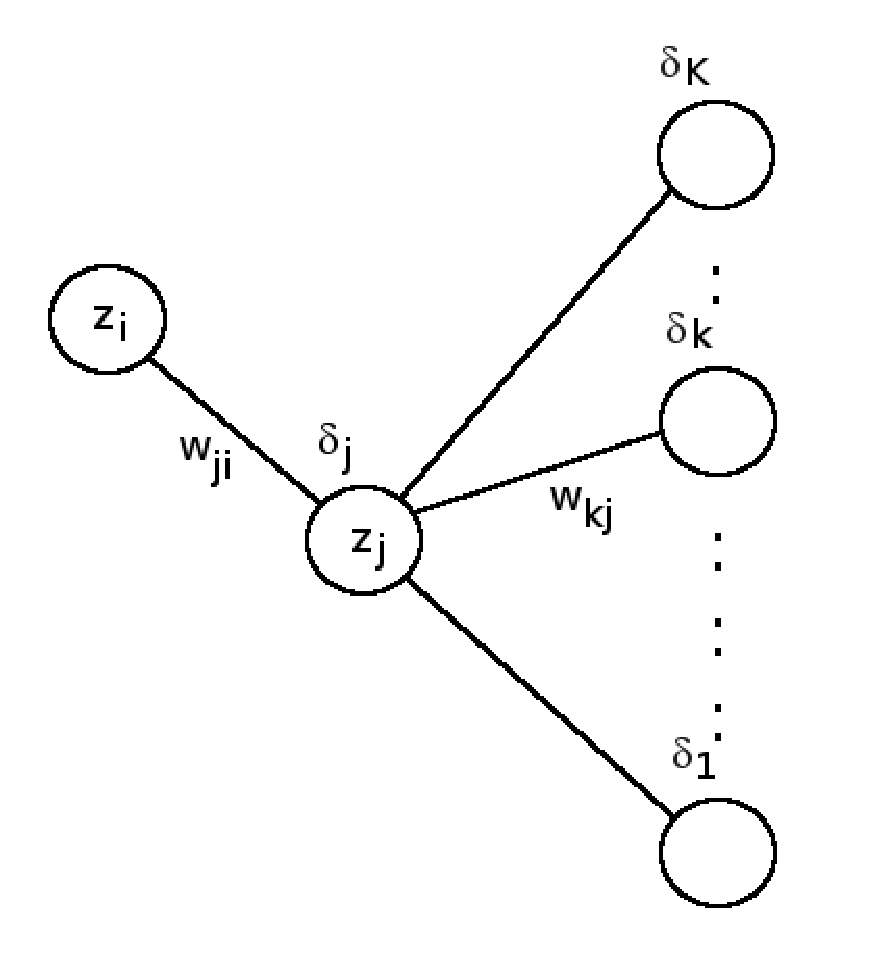
\includegraphics[height=3in]{04ANN/bpneurons.eps}
\end{center}
\caption{แสดงตัวแปร ในการทำ\textit{การแพร่กระจายย้อนกลับ} (backpropagation).}
\label{fig: ANN backprop}
\end{figure}
%

พิจารณา $\delta_k$ ของหน่วยเอาต์พุต, เราจะได้
\begin{eqnarray}
   \delta_k = y_k - t_k.
\label{eq: ANN BP delta k}   
\end{eqnarray}
ส่วน $\delta_j$ ของหน่วยซ่อน, เมื่อใช้กฎลูกโซ่ เราจะได้
\begin{eqnarray}
   \delta_j = \frac{\partial E_n}{\partial a_j} 
   = \sum_k \frac{\partial E_n}{\partial a_k} \cdot \frac{\partial a_k}{\partial a_j}
\label{eq: ANN BP delta j early}   
\end{eqnarray}
เมื่อ $a_k$ แทนค่าการกระตุ้นของหน่วยย่อยต่างๆ ที่หน่วยซ่อนของ $a_j$ เชื่อมต่อผ่านไปสู่เอาต์พุต.
รูป~\ref{fig: ANN backprop} แสดงหน่วยย่อยและการเชื่อมต่อ.
สังเกตุ หน่วยย่อยที่ $j$ (วงกลมกลางรูป) ต่อผ่านหน่วยย่อย $1$ ถึง $K$ (วงกลมต่างๆ ทางขวา) ไปสู่เอาต์พุต.

เมื่อ แทนสมการ~\ref{eq: ANN BP delta k}, \ref{eq: ANN neural output}, และ \ref{eq: ANN neural activation} ลงในสมการ~\ref{eq: ANN BP delta j early} จะได้
\begin{eqnarray}
  \delta_j = h'(a_j) \sum_k w_{kj} \delta_k.
\label{eq: ANN BP delta j}
\end{eqnarray}

สมการ~\ref{eq: ANN BP delta j} คือ สมการ\textit{การแพร่กระจายย้อนกลับ} (ฺBackpropagation), 
ซึ่ง บอกว่า ค่าของ $\delta$ ของแต่ละหน่วยย่อย หาได้จากการแพร่กระจายย้อนกลับของ $\delta$ ต่างๆ จากหน่วยย่อยที่อยู่ลึกลงไป (ใกล้เอาต์พุต).
\textit{อัลกอริทึ่มแพร่กระจายย้อนกลับ} (Error Backpropagation หรือ เรียกย่อๆ Backpropagation) สรุปขั้นตอนการคำนวณต่างๆ ดังนี้
\begin{itemize}
\item 1. ทำ\textit{การคำนวณไปข้างหน้า} (forward propagation), สมการ~\ref{eq: ANN neural activation} และ~\ref{eq: ANN neural output}
\item 2. คำนวณค่า $\delta_k$ สำหรับทุกๆหน่วยเอาต์พุต, สมการ~\ref{eq: ANN BP delta k}
\item 3. ทำแพร่กระจายย้อนกลับค่า $\delta$ ต่างๆ เพื่อคำนวณ $\delta_j$ ทุกหน่วยย่อย, สมการ~\ref{eq: ANN BP delta j}
\item 4. คำนวณค่าอนุพันธ์เป้าหมาย, สมการ~\ref{eq: ANN BP dE/dw}.
\end{itemize}

อัลกอริทึ่มแพร่กระจายย้อนกลับ เป็นวิธีการคำนวณค่าอนุพันธ์ของฟังชั่นจุดประสงค์สำหรับโครงข่ายประสาทเทียมที่มีประสิทธิภาพ
และครอบคลุมการคำนวณสำหรับโครงข่ายประสาทเทียมที่มีจำนวนชั้นหลายๆชั้นได้.
ค่าอนุพันธ์ของฟังชั่นเป้าหมายนี้สามารถนำไปใช้ประกอบกับวิธีการหาค่าตัวทำดีที่สุด 
เพื่อหาค่าน้ำหนักที่เหมาะสมสำหรับโครงข่ายประสาทเทียมได้.
บทที่~\ref{chapter: Applications of ANN} อภิปรายตัวอย่างการประยุกต์ใช้ทฤษฎีของโครงข่ายประสาทเทียมที่ถกในบทนี้
รวมถึงนำเสนอตัวอย่างโปรแกรมภาษาอาร์โปรเจคที่นำคณิตศาสตร์ที่พัฒนาขึ้นมานี้ไปสร้างเป็นโปรแกรม.


{\small
\begin{shaded}
\paragraph{\small เกร็ดความรู้จิตและการเรียนรู้}
(เรียบเรียงจาก \cite{Wikipedia}, \cite{AccessInsight}, และ \cite{Poo2010a})\\
%"All things are preceded by the mind, led by the mind, created by the mind." 
%Mind precedes all mental states. Mind is their chief; they are all mind-wrought.
``ทุกสิ่งเริ่มที่จิต นำโดยจิต และสร้างโดยจิต'' ธรรมบท\cite{AccessInsight}\\
\index{Mind}\index{จิต}

% Five Aggregates (ขันธ์ 5): 
% 1. รูป rupa = body
% 2. วิญญาณ vijnana = primary conciousness = Awareness, experience, in the sense that the presence of consciousness together with the sense organ and the object of the sense organ produces a sense experience or awareness.
% 3. สัญญา samjna = perception = the five sense consciousnesses (smell, touch, taste, seeing and hearing) and mental consciousness, in other words, direct perception. Perception also refers to the activity of recognition, or identification, such as attaching a name to an object of experience. It includes the formulation of a concept about a particular object.
% 4. เวทนา vedana = feelings = this refers only to the mental separation of perceptions into pleasant, unpleasant and neutral (nothing more).
% 5. สังขาร sankhara =  these are all other remaining mental processes, in general "thoughts"
จิตคือสภาวะเชิงการรับรู้และเชิงสติปัญญา ซึ่งรวมถึง 
สติรู้ตัว
การรับรู้สัมผัส  
ความรู้สึก อารมณ์ 
การคิด การตัดสินใจ การจดจำ การรับประสบการณ์ การเรียนรู้ และการตอบสนองต่อสภาวะแวดล้อม.
ส่วนประกอบของจิตนั้น อาจจัดออกได้เป็น $4$ หมวด.
%กลุ่มได้คือ (1) สติรู้ตัว (2) การรับรู้ผ่านทางสัมผัส (3) ความรู้สึก และ (4) ความคิดและกระบวนการเชิงสติปัญญาอื่นๆ.
%
หมวดหนึ่ง %(1) 
\textit{วิญญาณ}(vijnana) ซึ่งคือ\textit{สติรู้ตัว}(conciousness).
หมวดสอง %(2)
\textit{สัญญา} (samjana) ซึ่งคือ\textit{การรับรู้}(perception) ผ่านสัมผัสทางการมองเห็น สัมผัสทางการได้ยิน สัมผัสทางการได้กลิ่น
สัมผัสการรับรส สัมผัสทางกาย และสัมผัสที่มาจากจิตเอง.
จิตเองก็มีสัมผัสเช่นกัน ดังตัวอย่างของ\textit{อาการแขนขาลวง} (phantom limps) ที่เกิดในผู้ที่เสียแขนหรือขาไป แต่ภายหลังยังรู้สึกคันหรือเจ็บที่แขนหรือขาที่ไม่มีอยู่.
แม้ว่าสาเหตุของอาการนี้ยังไม่มีคำอธิบายที่ทางการแพทย์ยอมรับร่วมกันอย่างกว้างขวาง
แต่นายแพทย์\textit{วิลายานุร์ รามาฉันทรัน} (Vilayanur S. Ramachandran)
อธิบายว่า สัมผัสที่รู้สึกนั้นมาจากประสาทส่วนที่เคยทำงานกับแขนหรือขาส่วนนั้นขาดสัญญาณที่เคยได้รับ
และอาจส่งสัญญาณออกมาทั้งๆที่ไม่ได้รับสัญญาณรับรู้จริงๆ.
จากทฤษฎีนั้น นายแพทย์รามาฉันทรันเสนอวิธีการบำบัดอาการแขนขาลวง
โดยออกแบบกระบวนการให้ผู้มีอาการได้ฝึกประสาทรับรู้ใหม่ ซึ่งพบว่าได้ผลดีมาก.
หากมองจากมุมมองทางวิศวกรรม สัญญาณที่ขาดหายไปจากแขนขาที่เสียไปนั้น 
%หากเส้นทางของสัญญาณไม่ได้มีการจัดการใหม่ 
อาจให้ผลในลักษณะคล้ายการที่วงจรไฟฟ้ารับอินพุตมาจากขั้วปลายที่ปล่อยลอยอยู่
ซึ่งขั้วปลายที่ปล่อยลอยอาจรับ\textit{สัญญาณรบกวน}(noise)เข้ามาแทนได้ 
การฝึกประสาทรับรู้ใหม่ ก็อาจคล้ายการต่อขั้วปลายนั้นลง\textit{กราวด์}(ground)เพื่อปิดสัญญาณรบกวนนั้นลง.
หมวดสาม
%(3) 
\textit{เวทนา} (vedana) ซึ่งคือ\textit{ความรู้สึก}(feeling) อารมณ์ ความชอบ ความไม่ชอบ ความวางเฉย.
และ
หมวดสี่ 
%(4) 
\textit{สังขาร} (sankhara) ซึ่งคือ\textit{การคิดและกระบวนการเชิงสติปัญญาอื่นๆ} (mental activity) 
ได้แก่ การตัดสินใจ การตอบสนองต่อสภาวะแวดล้อม การจดจำ การรับประสบการณ์ และการเรียนรู้.

นักประสาทวิทยาด้านสติปัญญาชั้นนำ รีเบกก้า แซก\cite{Saxe2012a} เชื่อว่า
รูปแบบของกิจกรรมทางไฟฟ้าของเซลล์ประสาทเกี่ยวข้องโดยตรงกับ%ความคิด ศีลธรรม และ
จิตของเรา
เพียงแต่วงการวิทยาศาสตร์ยังไม่รู้อะไรมากเกี่ยวกับจิตและความสัมพันธ์ระหว่างรูปแบบของกิจกรรมทางไฟฟ้าและจิต

จากมุมมองของกิจกรรมทางไฟฟ้า
การเรียนรู้ก็เหมือนการปรับเปลี่ยนวงจรหรือเปลี่ยนการเชื่อมต่อภายในวงจร ซึ่งส่งผลให้เกิดการปรับเปลี่ยนพฤติกรรมของกิจกรรมทางไฟฟ้า.
%(
%พฤติกรรมของกิจกรรมทางไฟฟ้าของเซลล์ประสาทนั้นสามารถจะปรับตัวได้
%ซึ่งคือการเรียนรู้นั่นเอง.
\textit{สภาพพลาสติกของระบบประสาท} (synaptic plasticity) คือ ความสามารถของระบบประสาทที่สามารถเพิ่มหรือลดความแข็งแรงของการเชื่อมต่อสัญญาณประสาทระหว่างเซลล์ได้.
สภาพพลาสติกของระบบประสาทนี้เชื่อว่าเป็นคุณสมบัติที่อยู่เบื้องหลังความสามารถในการจดจำและการเรียนรู้ของสมอง.
กลไกนี้เปรียบเทียบได้กับการปรับค่าน้ำหนักหรือการฝึกโครงข่ายประสาทเทียม
แต่ประเด็นหนึ่งที่ต่างกันก็คือ
การเปลี่ยนค่าน้ำหนักของโครงข่ายประสาทเทียมจะทำเฉพาะในขั้นตอนการฝึกโครงข่ายประสาทเทียม
และค่าน้ำหนักที่ดีแล้วจะถูกตรึงให้คงค่าเหล่านั้นไว้คงที่ขณะใช้งาน.
แต่ระบบประสาท(ทางชีวภาพ)จะเปลี่ยนแปลงตัวเองตลอดเวลา 
เปลี่ยนขณะเรียนรู้ เปลี่ยนขณะคิด เปลี่ยนขณะทำกิจกรรมต่างๆ เปลี่ยนขณะทำงาน เปลี่ยนขณะไม่ได้ทำงาน เปลี่ยนขณะเล่น เปลี่ยนขณะทำสิ่งที่มีประโยชน์ เปลี่ยนขณะพักผ่อน เปลี่ยนขณะนอนหลับ และที่สำคัญเปลี่ยนแม้แต่ขณะทำสิ่งที่เป็นโทษ เช่น เมื่อสิ่งที่เราคาดหวังไม่ได้ดั่งใจ แล้วเราไม่ชอบใจ ถ้าเราเลือกที่จะโกรธ สมองจะเรียนรู้การตอบสนองนั้น และ
เมื่อเราทำแบบนั้นบ่อยๆ เราก็จะกลายเป็นคนที่โกรธง่าย หรือกล่าวอย่างชัดเจนก็คือ เราฝึกสมองของเราให้เก่งที่จะอยู่ในสภาวะอารมณ์โกรธนั่นเอง.

กลไกเบื้องหลังการส่งสัญญาณของระบบประสาท
กล่าวโดยคร่าวๆก็คือ 
เมื่อสัญญาณจากนิวเคลียสของเซลล์ประสาทเดินทางถึงปลายแอกซอนซึ่งเป็นปลายสำหรับส่งสัญญาณออก
สัญญาณซึ่งถ่ายทอดมาในรูปความต่างศักดิ์จะทำให้\textit{ช่องไอออนที่ควบคุมด้วยแรงดันไฟฟ้า}(voltage-gated ion channel) ของปลายแอกซอนเปิดออก
ทำให้\textit{แคลเซียมไอออน} (calcium ion สัญญลักษณ์ $Ca^{2+}$) ซึ่งอยู่ในของเหลวรอบๆเซลล์ ไหลเข้าสู่ปลายแอกซอน.
แคลเซียมไอออนที่เข้าสู่ปลายแอกซอนจะทำปฏิกิริยากับโปรตีนและเอนไซม์ภายในแอกซอน
ซึ่งส่งผลให้เกิดการปล่อยสารสื่อประสาทออกมา.
สารสื่อประสาทที่ออกมา
จะมีบางโมเลกุลที่ได้จับกับรีเซปเตอร์ที่ปลายเดนไดรต์ ซึ่งปลายเดนไดรต์คือปลายประสาทที่นำสัญญาณเข้าสู่เซลล์ประสาทตัวที่จะรับสัญญาณ.
เมื่อรีเซปเตอร์จับกับสารสื่อประสาทแล้ว จะทำให้รีเซปเตอร์เปลี่ยนโครงสร้างซึ่งจะเปิดช่องให้ไอออนบวกไหลเข้าสู่เดนไดรต์ เมื่อไอออนบวกไหลเข้าสู่เดนไดรต์จะทำให้ความต่างศักดิ์ของเดนไดรต์จุดนั้นเปลี่ยนไป
ซึ่งความต่างศักดิ์นี้เองเป็นสัญญาณที่จะถ่ายทอดต่อไปยังนิวเคลียสของเซลล์ประสาท.

%เมื่อพิจารณาที่ตัวสารสื่อประสาท 
สารสื่อประสาทเป็นกลไกหลักในการช่วยส่งสัญญาณประสาทข้ามเซลล์ประสาท
แต่ตัวสารสื่อประสาทเองไม่ได้ถูกส่งเข้าไปในเดนไดรต์ของเซลล์ประสาทตัวรับ.
มันทำหน้าที่เสมือนช่วยเปิดประตูให้ไอออนบวกได้เข้าไปในปลายเดนไดรต์ดังที่ได้อธิบายไปข้างต้น.
หลังจากสารสื่อประสาทจับกับรีเซปเตอร์ได้สักพัก มันจะหลุดออกมา.
สารสื่อประสาททั้งที่พึ่งหลุดมาจากการจับกับรีเซปเตอร์และที่ยังไม่ได้จับกับรีเซปเตอร์เลยจะถูกกำจัดออกไปโดยกลไกหลายๆชนิด เช่น การทำลายทิ้ง หรือ การที่ปลายแอกซอนดึงสารสื่อประสาทเหล่านี้กลับเข้าไปภายในเพื่อนำกลับไปใช้ใหม่.

การเรียนรู้หรือการปรับความแข็งแรงของการเชื่อมต่อสัญญาณระหว่างเซลล์ประสาท
เกี่ยวข้องกับการปรับความสามารถในการรับส่งสัญญาณประสาทระหว่างเซลล์.
%
เมื่อกล่าวถึงสัญญาณประสาทโดยละเอียดขึ้น 
สัญญาณประสาทจะถูกส่งในหลายรูปแบบ ขณะที่สัญญาณประสาทส่งผ่านเส้นทางจากนิวเคลียสของเซลล์ประสาทตัวหนึ่งไปสู่นิวเคลียสของเซลล์ประสาทอีกตัวหนึ่ง
มีการเปลี่ยนรูปแบบอยู่หลายครั้ง.
เมื่อเซลล์ประสาทอยู่ในสถานะถูกกระตุ้น นิวเคลียสของเซลล์จะส่งสัญญาณออกมาในรูปความถี่ของพัลส์.
นั่นคือ นิวเคลียสของเซลล์ประสาทจะส่งสัญญาณในลักษณะ\textit{พัลส์}(pulse) ซึ่งมักเรียกว่า\textit{ศักยะงาน} (action potential) 
เช่น ค่าความต่างศักย์ภายในเซลล์ประสาทจะมีค่าประมาณ $-70$ มิลลิโวลต์เมื่อเทียบกับจุดภายนอกเซลล์
แต่เมื่อมีศักยะงานเกิดขึ้น ค่าความต่างศักย์นี้เพิ่มขึ้นอย่างรวดเร็วจากค่าพักตัวที่ประมาณ $-70$ มิลลิโวลต์
ไปสูงสุดที่ประมาณ $40$ มิลลิโวลต์ หลังจากนั้นจะลดค่าลงอย่างรวดเร็วมาที่ราวๆ $-90$ มิลลิโวลต์ และกลับมาจบที่ค่าพักตัวที่ประมาณ $-70$ มิลลิโวลต์
โดยที่ศักยะงานแต่ละลูกจะยาวนานประมาณ $4$ มิลลิวินาที.
ความถี่หรือจำนวนศักยะงานต่อวินาทีจะขึ้นกับความแรงของสถานะการกระตุ้นของเซลล์ 
เช่น \textit{เซลล์โอล์แฟกตอรีคอร์เท็กซ์ไพรามิดอล} (Olfactory Cortex pyramidal cell) ที่ทำงานเกี่ยวกับการรับรู้กลิ่น จะส่งศักยะงานออกมาที่ความถี่ประมาณ $0.8$ ถึง $2.0$ ลูกต่อวินาที ขณะหายใจปกติ 
แต่จะส่งศักยะงานความถี่ประมาณ $4$ ถึง $11$ ลูกต่อวินาที ขณะที่เรากำลังดมอะไรอยู่\cite{NeuroBank}.
สัญญาณในรูปความถี่นี้ได้มีการศึกษามาตั้งแต่ ค.ศ. 1926 ที่ เอเดรียนและโซตเตอมัน\cite{AdrianZotterman1926a}
รายงานการศึกษาการกระตุ้นและสัญญาณไฟฟ้าเซลล์ประสาท
โดยใช้ตุ้มน้ำหนักดึงกล้ามเนื้อของกบและวัดสัญญาณไฟฟ้าจากเนื้อเยื้อประสาทของมัน
และพบความสัมพันธ์ที่ชัดเจน ระหว่างค่าน้ำหนักที่ยืดกล้ามเนื้อออก (ตัวแทนของปริมาณความแรงของการกระตุ้น)
กับความถี่ของศักยะงานที่เกิดขึ้น.
%แต่\textit{ขนาด}(magnitude)ของศักยะงานมีค่าประมาณคงที่ และไม่พบว่าเกี่ยวข้องกับความแรงของการกระตุ้นเลย.
ศักยะงานนี้คือสัญญาณที่ถูกส่งออกจากนิวเคลียสผ่านไปที่ปลายแอกซอน
สัญญาณที่ส่งผ่านออกจากปลายแอกซอนของเซลล์ตัวส่งเข้าไปสู่ปลายเดนไดร์ตของเซลล์ตัวรับจะส่งผ่านกลไกของสารสื่อประสาท
และปลายเดนไดรต์รับสัญญาณประสาทเข้ามาในรูประดับความต่างศักย์ระหว่างภายในปลายเดนไดร์ตและภายนอก
ซึ่งรูปแบบที่เปลี่ยนไปของสัญญาณประสาทจากนิวเคลียสของตัวส่งไปจนถึงปลายแอกซอน(ในรูปศักยะงาน) ผ่านไซแนปซ์ (ในรูปสารสื่อประสาท) และรับเข้าสู่ปลายเดนไดร์ตไปจงถึงส่งเข้าไปสู่นิวเคลียสของตัวรับ (ในรูประดับความแรงของความต่างศักย์) เกี่ยวข้องสัมพันธ์กับทฤษฎีที่ใช้อธิบายกระบวนการเรียนรู้เซลล์ประสาท.

%เซลล์โอล์แฟกตอรีคอร์เท็กซ์ไพรามิดอล (Olfactory Cortex pyramidal cell) 
%& olfactory cortex
%& Glutamate 
%Individual pyramidal cell spike trains represent input associated with the theta rhythm (3-12 Hz), respiration (0.8-2.0 Hz), exploratory sniffing (4-11 Hz) and the mean spike rates of olfactory bulb mitral cells (3-20 Hz)

ทฤษฎีที่อธิบายการปรับความแข็งแรงของการเชื่อมต่อสัญญาณระหว่างเซลล์ประสาท
กล่าวถึง กลไกหลัก $2$ กลไก.
นั่นคือ \textit{การเพิ่มความแข็งแรงเชิงประสาทระยะยาว} (long-term synaptic potentiation คำย่อ LTP) และ \textit{การถดถอยความแข็งแรงเชิงประสาทระยะยาว} (long-term synaptic depression คำย่อ LTD).
จากงานศึกษาการเชื่อมต่อของเซลล์ในฮิปโปแคมปัส โดยเฉพาะไซแนปส์ที่เชื่อมต่อระหว่างเซลล์ประสาทในบริเวณ\textit{ซีเอ3} (CA3) ที่ส่งแอกซอน (ซึ่งเรียกว่า \textit{แชฟเฟอร์คอแลทเตอรอล} Schaffer collaterals) ไปเชื่อมต่อกับเซลล์ประสาทในบริเวณซีเอ1 
สรุปว่า
เมื่อมีการกระตุ้นด้วยสัญญาณประสาทความถี่สูงผ่านไซแนปส์ ค่าความต่างศักย์ที่ได้รับที่ปลายเดนไดรต์ของไซแนปส์นั้นจะมีค่าเพิ่มขึ้นมาก และค่านั้นจะคงอยู่เป็นเวลานาน (หลายนาทีหรือหลายวัน หลังจากการกระตุ้นนั้น)
โดยค่าความต่างศักย์ที่ปลายเดนไดรต์ที่เชื่อมต่อไซแนปส์อื่นจะไม่ได้รับผลกระทบ.
สิ่งนี้เรียกว่า การเพิ่มความแข็งแรงเชิงประสาทระยะยาว.
และในทางกลับกัน
เมื่อมีการกระตุ้นด้วยสัญญาณประสาทความถี่ต่ำผ่านไซแนปส์ ค่าความต่างศักย์ที่ได้รับที่ปลายเดนไดรต์ของไซแนปส์นั้นจะมีค่าลดลงมาก และค่านั้นก็คงอยู่เป็นเวลานาน
โดยค่าความต่างศักย์ที่ปลายเดนไดรต์ที่เชื่อมต่อไซแนปส์อื่นจะไม่ได้รับผลกระทบ.
สิ่งนี้เรียกว่า การถดถอยความแข็งแรงเชิงประสาทระยะยาว.
ประเด็นสำคัญ คือ (1) มีการเปลี่ยนแปลงความแข็งแรงของไซแนปส์ระยะยาวเกิดขึ้น
(2) ผลการเปลี่ยนแปลงความแข็งแรงขึ้นกับความถี่
(3) ผลการเปลี่ยนแปลงเกิดขึ้นเฉพาะตัวของไซแนปส์.

กลไกเบื้องหลัง%
%ทั้งการเพิ่มความแข็งแรงเชิงประสาทระยะยาวและการถดถอยความแข็งแรงเชิงประสาทระยะยาว
นั้นอธิบายว่า
ไซแนปส์ของแชฟเฟอร์คอแลทเตอรอล ทำงานผ่านสารสื่อประสาทกลูตาเมท
และปลายประสาทของเซลล์ตัวรับที่ซีเอ1มีรีเซปเตอร์ที่ทำงานกับกลูตาเมทอยู่ $2$ ชนิด คือ \textit{แอมปารีเซปเตอร์} (AMPA receptor) และ \textit{เอนเอมดีเอรีเซปเตอร์} (NMDA receptor).
เมื่อปลายประสาทของเซลล์ที่ซีเอ3จะส่งสัญญาณกระตุ้นส่งผ่านไซแนปส์ 
มันจะปล่อยสารสื่อประสาทกลูตาเมทออกมา.
เมื่อกลูตาเมทจับกับแอมปารีเซปเตอร์ แอมปารีเซปเตอร์จะเปิดออก 
และด้วยคุณสมบัติของแอมปารีเซปเตอร์ โซเดียมไอออนจะไหลเข้าสู่ปลายเดนไดรต์ตัวรับที่ซีเอ1
แคลเซียมไอออนบางส่วนก็อาจไหลเข้าได้บ้างแต่ไม่มาก.
แอมปารีเซปเตอร์ที่เปิดรับโซเดียมไอออนแล้วซักพักก็จะปิดลง.
%
เมื่อกลูตาเมทจับกับเอนเอมดีเอรีเซปเตอร์ เอนเอมดีเอรีเซปเตอร์จะเปิดออกเช่นกัน แต่เอนเอมดีเอรีเซปเตอร์จะมีแมกนีเซียมไอออนปิดช่องอยู่ ทำให้ไอออนยังไม่สามารถไหลผ่านได้.
หลังจากโซเดียมไอออนผ่านแอมปารีเซปเตอร์เข้าสู่เซลล์ซีเอ1
สักพักปริมาณโซเดียมไอออนจะถูกสูบออกโดยกลไกของ\textit{โซเดียม-โปแตสเซียมปั๊ม} (sodium-potassium pump) ซึ่งเป็นเอนไซมน์ที่ทำงานรักษาสมดุลของเซลล์.

\paragraph{\small การเพิ่มความแข็งแรงเชิงประสาทระยะยาว}
หากการกระตุ้นมีความถี่สูงพอที่โซเดียมไอออนที่ไหลเข้ามาจะสะสมได้ (ความถี่สูงพอที่จะสะสมโซเดียมไอออน ที่เหลือจากการสูบออกของโซเดียม-โปแตสเซียมปั๊ม)
ปริมาณโซเดียมไอออนที่เพิ่มขึ้นมาก จะทำให้เกิดไฟฟ้าสถิตย์ที่มากพอจะผลักแมกนีเซียมไอออนที่ปิดเอนเอมดีเอรีเซปเตอร์ออกไปได้.
เมื่อแมกนีเซียมหลุดออกไป แคลเซียมไอออนก็สามารถผ่านเข้ามาทางเอนเอมดีเอรีเซปเตอร์ได้.
แคลเซียมไอออนที่ไหลเข้าปริมาณมากจะช่วยเพิ่มค่าความต่างศักย์ที่ได้รับที่ปลายเดนไดรต์ขึ้นไป.
นอกจากนั้นแคลเซียมไอออนปริมาณมากจะจับกับ\textit{โปรตีนคีเนส} (Protein kinases) ซึ่งส่งผลให้เกิดการประกอบแอมปารีเซปเตอร์และติดแอมปารีเซปเตอร์เข้าไปทำงานที่ปลายเชื่อมประสาทเพิ่มขึ้น.
ผลการเพิ่มแอมปารีเซปเตอร์จากกระบวนการนี้จะคงอยู่เพียงแค่เวลาสั้นๆไม่กี่ชั่วโมงเท่านั้น
%แต่หากแคลเซียมไอออนปริมาณมากนี้เกิดเพียงช่วงสั้นๆ (การตุ้นด้วยสัญญาณความถี่สูง ในระยะเวลาสั้นๆ) 
%และ
แต่หากมีแคลเซียมไอออนไหลเข้ามาในปริมาณมากเป็นระยะเวลานานพอ (มีการกระตุ้นด้วยสัญญาณประสาทความถี่สูงเป็นระยะเวลานาน) จะส่งผลต่อเนื่องไปจนทำให้เกิดการเพิ่ม\textit{ปัจจัยการลอกรหัสดีเอ็นเอ} (transcription factor) ซึ่งส่งผลต่อ\textit{การแสดงออกของยีน} (gene expression) และทำให้เกิดการสร้างโปรตีนที่ทำให้เกิดทั้งแอมปารีเซปเตอร์ใหม่เพิ่มขึ้น และ \textit{โกรทแฟคเตอร์} (growth factor) ที่จะไปทำให้เกิดการสร้างไซแนปส์ใหม่เพิ่มขึ้น ซึ่งผลจากกระบวนการนี้จะยาวนานและคงทนมาก.

\paragraph{\small การถดถอยความแข็งแรงเชิงประสาทระยะยาว}
สำหรับการกระตุ้นที่มีความถี่ต่ำ จะส่งผลให้ปริมาณของแคลเซียมไอออนอยู่ในระดับต่ำ.
ปริมาณของแคลเซียมไอออนที่อยู่ในระดับต่ำจะไปกระตุ้นการทำงานของเอนไซม์\textit{ฟอสเฟตเตส} (phosphatase)
ซึ่งส่งผลไปลดจำนวนแอมปารีเซปเตอร์ที่ทำงานได้ลง.

การเพิ่มความแข็งแรงเชิงประสาทระยะยาว และ การถดถอยความแข็งแรงเชิงประสาทระยะยาว ต่างก็มีปัจจัยมาจากปริมาณแคลเซียมไอออนในปลายไซแนปส์ตัวรับ
โดย ปริมาณแคลเซียมไอออนในระดับสูงจะทำให้เกิดการเพิ่มความแข็งแรงเชิงประสาทระยะยาว
และ ปริมาณแคลเซียมไอออนในระดับต่ำจะทำให้เกิดการถดถอยความแข็งแรงเชิงประสาทระยะยาว.
%
ระดับที่เป็นขีดแบ่งระหว่างการเพิ่มและการถดถอยนี้
เชื่อว่าน่าจะเปลี่ยนแปลงตามสภาวะของเซลล์ในลักษณะที่ช่วยรักษาสมดุลย์
(\textit{ทฤษฎีบีซีเอ็ม} BCM theory\cite{BCM1982})
ได้แก่
การเปลี่ยนแปลงในลักษณะ\textit{การป้อนกลับเชิงลบ} (negative feedback)
เช่น
เมื่อไซแนปส์อยู่ในภาวะการเพิ่มความแข็งแรงเชิงประสาทระยะยาว ระดับขีดแบ่งนี้น่าจะสูงขึ้นเพื่อช่วยลดความเสี่ยงของการเพิ่มมหาศาลลง
และ เมื่อไซแนปส์อยู่ในภาวะการถดถอยความแข็งแรงเชิงประสาทระยะยาว ระดับขีดแบ่งนี้น่าจะลดลงเพื่อช่วยลดความเสี่ยงของการถดถอยจนสูญเสียการเชื่อมต่อ.

จากสภาพพลาสติกของระบบประสาทและทฤษฎีบีซีเอ็ม
เราอาจกล่าวได้ว่า การเรียนรู้ที่มีประสิทธิภาพคือ
การเรียนรู้ต่อเนื่อง สลับกับการหยุดพักผ่อน
เพื่อให้เกิดการกระตุ้นประสาทต่อเนื่องยาวนานเพียงพอ ที่จะทำให้เกิดการสร้างการเชื่อมต่อใหม่
และ หยุดพักเพื่อให้ระดับขีดแบ่งปรับตัวลงมา ทำให้การสร้างการเชื่อมต่อใหม่ทำได้ง่ายขึ้น
เพราะ การเรียนรู้ต่อเนื่องเป็นเวลานานเกินไป จะเพิ่มระดับขีดแบ่งซึ่งจะทำให้การเข้าสู่ภาวะการเพิ่มความแข็งแรงเชิงประสาทระยะยาวทำได้ยากขึ้น.
\\

%\setlength{\parindent}{0cm}
%\begin{tabular}{ll}
\hspace{-0.4in}
\begin{tabular}{ >{\arraybackslash}m{2.7in}  >{\arraybackslash}m{2.8in} }
``Never go to excess, but let moderation be your guide.''
&
``ทำสิ่งใดอย่ามากเกินไป ให้ความพอดีเป็นตัวชี้ทาง''
\\
Marcus Tullius Cicero
&
มาร์คัส ทูลลิอุส ซิเซอโร
\end{tabular} 
%\setlength{\parindent}{default}

%อออนที่ปิดเอนเอมดีเอรีเซปเตอร์อยู่ เมื่อเอนเอมดีเอรีเซปเตอร์จับกับ

%มีโอกาสจะจับกับกลูตาเมทรอบใหม่และเปิดออกเพื่อรับโซเดียมไอออนเข้าไปเพิ่ม
%ปริมาณของโซเดียมไอออนที่เข้าไปเป็นจำนวนมากในช่วงเวลาสั้นๆ จะ


%หากการกระตุ้นมีความถี่ต่ำปริมาณโซเดียมและ


%ทั้งแอมปารีเซปเตอร์และเอนเอมดีเอรีเซปเตอร์นั้นยอมให้แคลเซียมไอออนสามารถผ่านได้
%แต่เอนเอมดีเอรีเซปเตอร์นั้นยอมให้แคลเซียมไอออนสามารถผ่านได้ดีกว่าแอมปารีเซปเตอร์มาก
%เพียงแต่เอนเอมดีเอรีเซปเตอร์จะมีแมกนีเซียมไอออนปิดช่องอยู่.






%หรือมักเรียกว่า อีพีเอสพี (Excitatory postsynaptic potential คำย่อ EPSP)


%คำอธิบายกลไกเบื้องหลังของการเพิ่มความแข็งแรงเชิงประสาทระยะยาว และการถดถอยความแข็งแรงเชิงประสาทระยะยาว
%ได้มาจากการอนุมานความรู้ที่ได้จากงานวิจัยต่างๆ ที่ศึกษาการเชื่อมต่อของเซลล์ในฮิปโปแคมปัส โดยเฉพาะการเชื่อมต่อระหว่างเซลล์ประสาทในบริเวณ\textit{ซีเอ3} (CA3) ที่ส่งแอกซอน (ซึ่งเรียกว่า \textit{แชฟเฟอร์คอแลทเตอรอล} Schaffer collaterals) ไปเชื่อมต่อกับเซลล์ประสาทในบริเวณซีเอ1.
%งาน
%สรุปได้ความว่า



%งานที่เป็นต้นแบบของงานศึกษาการเพิ่มความแข็งแรงเชิงประสาทระยะยาว คืองานของบลิสกับโลโม\cite{BlissLomo1973} ที่ศึกษาสมองของกระต่ายในส่วนฮิปโปแคมปัส และพบว่าการกระตุ้นแอกซอนด้วยความถี่สูงในช่วงสั้นๆ จะส่งผลให้การเชื่อมต่อที่ไซแนปส์ระหว่างแอกซอนนั้นกับเดนไดรต์ของเซลล์ตัวรับแข็งแรงขึ้น.





%Most neuronal AMPARs contain this critical subunit (GluR2)
%AMPA with GluR2 subunit is impermeable to Calcium ion.
%(Why? 
%Calcium ion is about the same size as sodium ion (Ca++ 114pm c.f. Na+ 116pm)
%)

%Double bouquet cell
%& visual cortex 
%& GABA


%CA1 pyramidal neuron
%& CA1, hippocampus
%& Glutamate


%[Jennifer Aniston neurons]


%[ความสุขและศาสนา]

%เซลล์[ตัวอย่าง /อ้างอิง] เมื่อไม่อยู่ในสถานะถูกกระตุ้นจะส่งศักยะงานนี้ออกมาประมาณ ... ลูกต่อวินาที
%ส่วนเซลล์ที่ถูกกระตุ้นจะส่งศักยะงานนี้ออกมาประมาณ ... ลูกต่อวินาที

%https://en.wikipedia.org/wiki/Neural_coding

%ใครเจอ ... LTP ...
%[LTP/LTD]

%http://neuroscience.uth.tmc.edu/s1/chapter07.html

%There are two general forms of synaptic plasticity, intrinsic and extrinsic. Intrinsic mechanisms, also known as homosynaptic mechanisms, refer to changes in the strength of a synapse that are brought about by its own activity. (Homo from the Greek meaning the same.) Extrinsic plasticity, or heterosynaptic plasticity, is a change in the strength of a synapse brought about by activity in another pathway.

%...
%[vdo synaptic plasticity]
%[vdo neuroscience LTP]


%[neuroplasticity]
%https://en.wikipedia.org/wiki/Neuroplasticity
%
%https://en.wikipedia.org/wiki/Long-term_potentiation

%In neuroscience, long-term potentiation (LTP) is a persistent strengthening of synapses based on recent patterns of activity. These are patterns of synaptic activity that produce a long-lasting increase in signal transmission between two neurons.[2] The opposite of LTP is long-term depression, which produces a long-lasting decrease in synaptic strength.
%It is one of several phenomena underlying synaptic plasticity, the ability of chemical synapses to change their strength. As memories are thought to be encoded by modification of synaptic strength,[3] LTP is widely considered one of the major cellular mechanisms that underlies learning and memory.[2][3]
%LTP was discovered in the rabbit hippocampus by Terje Lømo in 1966 and has remained a popular subject of research since. Many modern LTP studies seek to better understand its basic biology, while others aim to draw a causal link between LTP and behavioral learning. Still others try to develop methods, pharmacologic or otherwise, of enhancing LTP to improve learning and memory. LTP is also a subject of clinical research, for example, in the areas of Alzheimer's disease and addiction medicine.

\end{shaded}
}%small

%[Pheneas Gage]
%[RTPj]

%But, we know much less about is how [would] a pattern of electrical activity in a brain cell relates to thinking about morality. 

%What pattern of activity is it ...
 
%[brain to mind]
%สมองกับจิตใจ

%http://www.scientificamerican.com/article/electrical-circuits-encode-your-reality/
% c.f. role of neurotransmitters

%{\small
%\begin{shaded}
%\paragraph{\small เกร็ดความรู้กลไกการส่งสัญญาณประสาท}
%(เรียบเรียงจาก \cite{BuddhasBrain} และ \cite{Wikipedia})

%https://en.wikipedia.org/wiki/Action_potential
%โดยทั่วๆไปแล้ว ความต่างศักย์ภายในเซลล์ของมนุษย์จะมีค่าประมาณ $-70$ mV เมื่อเทียบกับภายนอกเซลล์ ความต่างศักย์นี้เรียกว่า \textit{ความต่างศักย์เมมเบรน} (membrane potential).
%เซลล์หลายชนิดจะมีค่าความต่างศักย์เมมเบรนค่อนข้างคงที่
%แต่ค่าความต่างศักย์เมมเบรนของเซลล์ประสาทไม่คงที่ %และเปลี่ยนแปลงบ่อยๆในลักษณะของการเพิ่มขึ้นของรวดเร็วและตามด้วยการลดลงอย่างรวดเร็ว
%รอบของการเพิ่มและลดของค่าความต่างศักย์เมมเบรนของเซลล์ประสาทนี้จะเรียกว่า \textit{ศักยะงาน} (action potential)


%\paragraph{\small สารสื่อประสาท}
%[Neurotransmitter]
%สารสื่อประสาทมีหลากหลายชนิด
%แต่ละชนิดทำหน้าที่ต่างๆกัน

%check if ratio of neurotransmitter intake is actually the connection strength.
%https://en.wikipedia.org/wiki/Chemical_synapse#Synaptic_strength

%An electrochemical wave called an action potential travels along the axon of a neuron. When the action potential reaches the presynaptic terminal, it provokes the release of a small quantity of neurotransmitter molecules, which bind to chemical receptor molecules located in the membrane of another neuron, the postsynaptic neuron, on the opposite side of the synaptic cleft.
 

%\end{shaded}
%}


\section{แบบฝึกหัด}
\label{section: ANN exercises}

\paragraph{1.} 
จงแสดงให้เห็นว่าอนุพันธ์ของสมการ~\ref{eq: ANN En 2-layer regression} 
คือสมการ~\ref{eq: ANN dEn/w2 0}, \ref{eq: ANN dEn/w2 i}, \ref{eq: ANN dEn/w1 0}, และ \ref{eq: ANN dEn/w1 i}.
และจงแสดงให้เห็นว่าอนุพันธ์ของ $h(a) = \frac{1}{1 + \exp(-a)}$ คือ
$h'(a) = h(a) \cdot (1 - h(a))$.

\paragraph{2.}
จงแสดงให้เห็นว่า $\frac{\partial E_n}{\partial a_k} = y_k - t_k$
เมื่อฟังชั่นกระตุ้นของโครงข่ายชั้นเอาต์พุตและฟังชั่นเป้าหมายเป็นดังนี้
\begin{itemize}
\item (ก) สำหรับการหาค่าถดถอย เอาต์พุตเป็น\textit{ฟังชั่นเอกลักษณ์} (identity function) ซึ่งคือ $y_k = a_k$ และ\textit{ฟังชั่นค่าใช้จ่าย} (cost function) คือ $\mathrm{Cost}_n = \frac{1}{2} \sum_k (y_k - t_{kn})^2$.
\item (ข) สำหรับการจำแนกประเภทแบบสองกลุ่ม เอาต์พุตเป็น\textit{ฟังชั่นซิกมอยด์} (sigmoid function) ซึ่งคือ $y_1 = \frac{1}{1 + \exp(-a_1)}$ และ\textit{ฟังชั่นค่าใช้จ่าย}คือ $\mathrm{Cost}_n = - t_n \log (y_1) - (1-t_n) \log(1-y_1)$.
\item (ค) สำหรับการจำแนกประเภทแบบหลายกลุ่ม เอาต์พุตเป็น\textit{ฟังชั่นซอฟต์แมกซ์} (softmax function) ซึ่งคือ $y_k = \frac{\exp(a_k)}{\sum_{q=1}^K \exp(a_q)}$ 
และ\textit{ฟังชั่นค่าใช้จ่าย}คือ $\mathrm{Cost}_n = - \sum_k t_{kn} \log (y_k)$.
\end{itemize}

\paragraph{3.}
จงแสดงว่าสมการ~\ref{eq: ANN BP delta j} ได้มาจากสมการ~\ref{eq: ANN BP delta j early}.

\paragraph{4.}
โครงข่ายประสาทเทียมก็สามารถทำเรกูลาไรเซชั่นได้เช่นเดียวกับโมเดลเชิงเส้น (หัวข้อ~\ref{sec: regularization}).
จากฟังชั่นเป้าหมายสำหรับการหาค่าถดถอย (สมการ~\ref{eq: ANN error function}), เทอมสำหรับเรกูลาไรเซชั่นสามารถเพิ่มเข้าไปได้เป็น
%\begin{eqnarray}
%   E(\mathbf{w}) &=& \frac{1}{2} \sum_{n=1}^N \Vert \mathbf{y}(\mathbf{x}_n, \mathbf{w}) - \mathbf{t}_n \Vert^2 + \frac{\lambda}{2} \mathbf{w}^T \mathbf{w}
%\label{eq: ann regularized error function}   
%\end{eqnarray}
%ดังนั้น,
\begin{eqnarray}
   \mathbf{Cost}_n &=& E_n + \frac{\lambda_1}{2} \sum_{i \neq 0} ( w_{ji}^{(1)} )^2 + \frac{\lambda_2}{2} \sum_{j \neq 0} ( w_{kj}^{(2)} )^2
%   
%   \frac{1}{2} \sum_{k=1}^K \left\{ y_k - t_{k,n} \right\}^2 + \frac{\lambda_1}{2} \sum_{w \in \mathbf{W}_1} w^2 + \frac{\lambda_2}{2} \sum_{w \in \mathbf{W}_2} w^2
\label{eq: ann regularized En}   
\end{eqnarray}
สังเกตุว่าเรกูลาไรเซชั่นเทอมไม่รวมค่าไบอัส ($w_{j0}^{(1)}$, $w_{k0}^{(2)}$).
จงแสดงให้เห็นว่า
\begin{eqnarray}
\frac{\partial \mathbf{Cost}_n}{\partial w_{ji}^{(1)}} &=& \frac{\partial E_n}{\partial w_{ji}^{(1)}} + \lambda_1 w_{ji}^{(1)}
\label{eq: ann regularized derivative 1} \\
\frac{\partial \mathbf{Cost}_n}{\partial w_{kj}^{(2)}} &=& \frac{\partial E_n}{\partial w_{kj}^{(2)}} + \lambda_2 w_{kj}^{(2)}.
\label{eq: ann regularized derivative 2}
\end{eqnarray}

\paragraph{5.}
จากสมการ~\ref{eq: ANN lin model}
%จงยกตัวอย่าง โมเดลที่มีเบซิสฟังชั่นที่เป็นฟังชั่นเชิงเส้นกับ $\mathbf{x}$
%นั่นคือ $\phi_j(\mathbf{x}) = c_0 x_0 + c_1 x_1 + \cdots + c_D x_D$ 
%โดย
%สมมติข้อมูลและหาค่าพารามิเตอร์ของโมเดลเพื่อทำนายข้อมูล
%และศึกษาความสัมพันธ์ระหว่าง $y$ กับ $\mathbf{x}$
%เปรียบเทียบกับ โมเดลที่มีเบซิสฟังชั่น $\phi_j(\mathbf{x}) = x_j$
จงอภิปรายความเหมือนและความต่าง ในเชิงความสามารถในการประมาณความสัมพันธ์ข้อมูล
ระหว่างโมเดลที่มีเบซิสฟังชั่นที่เป็นฟังชั่นเชิงเส้นกับอินพุต
และโมเดลที่มีเบซิสฟังชั่นเป็นอินพุตตรงๆ (นั่นคือ $\phi_j(\mathbf{x}) = x_j$)
พร้อมยกตัวอย่างให้เห็นภาพ
และจงอภิปรายถึงเหตุผลของการเลือกเบซิสฟังชั่นที่ต้องไม่เป็นฟังชั่นเชิงเส้นกับอินพุต ดังกล่าวในตอนต้นของหัวข้อ~\ref{sec: ANN structure}

\paragraph{6.}
จงหาข้อมูลและเปรียบเทียบโครงข่ายประสาทเทียมกับวิธี\textit{ซับเพอร์เวคเตอร์แมชชีน}(support vector machine)\cite{CortesVapnik1995a}
และวิธี\textit{ป่าสุ่ม}(random forest)\cite{Breiman2001a} ในเชิงฟังชั่นจุดประสงค์
และการคำนวณเพื่อทำนายกลุ่ม และกระบวนการในการคำนวณค่าน้ำหนัก
พร้อมอภิปรายข้อดีข้อเสียของทั้งสามวิธี

\paragraph{7.}
จงหาข้อมูลการพัฒนาและผู้เชี่ยวชาญที่มีส่วนสำคัญในการพัฒนาของโครงข่ายประสาทเทียม 
วิธีซับเพอร์เวคเตอร์แมชชีน
และวิธีป่าสุ่ม.
และจงอภิปรายสิ่งที่ได้เรียนรู้จากการศึกษาประวัติการพัฒนาของวิธีการต่างๆ รวมถึงวิธีการทำงานของผู้เชี่ยวชาญที่มีส่วนสำคัญในการพัฒนาของวิธีการเหล่านี้

\paragraph{8.}
จงหาข้อมูลของวิธีการเรียนรู้ของเครื่องแบบต่างๆ เช่น \textit{โครงข่ายแบบแผนที่จัดโครงสร้างตัวเอง} (self-organizing map)\cite{Kohonen1982a}, \textit{วิธีการกรองเชิงความร่วมมือ} (Collaborative Filtering)\cite{EkstrandEtAl2010a}, \textit{วิธีเคมีนส์} (K-Means)\cite{Bishop2006a}, \textit{วิธีการประมาณความหนาแน่นเชิงแก่น} (Kernel Density Estimation)\cite{Bishop2006a}, 
\textit{วิธีวิเคราะห์ส่วนประกอบหลัก} (Principle Component Analysis)\cite{Bishop2006a},
และ \textit{ซาซ่าอัลกอริทึ่ม} (SARSA algorithm)\cite{SuttonBarto1998a}
และจงอภิปรายภาระกิจของวิธีต่างๆเหล่านี้ จากมุมมองของศาสตร์การหาค่าดีที่สุด (บทที่~\ref{chapter: Optimization})
% $T$ ประสบการณ์ $E$ และ ดัชนีวัดสมรรถนะ $P$ 
พร้อมระบุฟังชั่นจุดประสงค์และตัวแปรตัดสินใจที่วิธีเหล่านี้กำหนดขึ้น

